\documentclass[]{book}
\usepackage{lmodern}
\usepackage{amssymb,amsmath}
\usepackage{ifxetex,ifluatex}
\usepackage{fixltx2e} % provides \textsubscript
\ifnum 0\ifxetex 1\fi\ifluatex 1\fi=0 % if pdftex
  \usepackage[T1]{fontenc}
  \usepackage[utf8]{inputenc}
\else % if luatex or xelatex
  \ifxetex
    \usepackage{mathspec}
  \else
    \usepackage{fontspec}
  \fi
  \defaultfontfeatures{Ligatures=TeX,Scale=MatchLowercase}
\fi
% use upquote if available, for straight quotes in verbatim environments
\IfFileExists{upquote.sty}{\usepackage{upquote}}{}
% use microtype if available
\IfFileExists{microtype.sty}{%
\usepackage{microtype}
\UseMicrotypeSet[protrusion]{basicmath} % disable protrusion for tt fonts
}{}
\usepackage{hyperref}
\hypersetup{unicode=true,
            pdftitle={African American Studies 188: Intro to R \& Mapping in R},
            pdfauthor={Tim Dennis},
            pdfborder={0 0 0},
            breaklinks=true}
\urlstyle{same}  % don't use monospace font for urls
\usepackage{natbib}
\bibliographystyle{apalike}
\usepackage{color}
\usepackage{fancyvrb}
\newcommand{\VerbBar}{|}
\newcommand{\VERB}{\Verb[commandchars=\\\{\}]}
\DefineVerbatimEnvironment{Highlighting}{Verbatim}{commandchars=\\\{\}}
% Add ',fontsize=\small' for more characters per line
\usepackage{framed}
\definecolor{shadecolor}{RGB}{248,248,248}
\newenvironment{Shaded}{\begin{snugshade}}{\end{snugshade}}
\newcommand{\AlertTok}[1]{\textcolor[rgb]{0.94,0.16,0.16}{#1}}
\newcommand{\AnnotationTok}[1]{\textcolor[rgb]{0.56,0.35,0.01}{\textbf{\textit{#1}}}}
\newcommand{\AttributeTok}[1]{\textcolor[rgb]{0.77,0.63,0.00}{#1}}
\newcommand{\BaseNTok}[1]{\textcolor[rgb]{0.00,0.00,0.81}{#1}}
\newcommand{\BuiltInTok}[1]{#1}
\newcommand{\CharTok}[1]{\textcolor[rgb]{0.31,0.60,0.02}{#1}}
\newcommand{\CommentTok}[1]{\textcolor[rgb]{0.56,0.35,0.01}{\textit{#1}}}
\newcommand{\CommentVarTok}[1]{\textcolor[rgb]{0.56,0.35,0.01}{\textbf{\textit{#1}}}}
\newcommand{\ConstantTok}[1]{\textcolor[rgb]{0.00,0.00,0.00}{#1}}
\newcommand{\ControlFlowTok}[1]{\textcolor[rgb]{0.13,0.29,0.53}{\textbf{#1}}}
\newcommand{\DataTypeTok}[1]{\textcolor[rgb]{0.13,0.29,0.53}{#1}}
\newcommand{\DecValTok}[1]{\textcolor[rgb]{0.00,0.00,0.81}{#1}}
\newcommand{\DocumentationTok}[1]{\textcolor[rgb]{0.56,0.35,0.01}{\textbf{\textit{#1}}}}
\newcommand{\ErrorTok}[1]{\textcolor[rgb]{0.64,0.00,0.00}{\textbf{#1}}}
\newcommand{\ExtensionTok}[1]{#1}
\newcommand{\FloatTok}[1]{\textcolor[rgb]{0.00,0.00,0.81}{#1}}
\newcommand{\FunctionTok}[1]{\textcolor[rgb]{0.00,0.00,0.00}{#1}}
\newcommand{\ImportTok}[1]{#1}
\newcommand{\InformationTok}[1]{\textcolor[rgb]{0.56,0.35,0.01}{\textbf{\textit{#1}}}}
\newcommand{\KeywordTok}[1]{\textcolor[rgb]{0.13,0.29,0.53}{\textbf{#1}}}
\newcommand{\NormalTok}[1]{#1}
\newcommand{\OperatorTok}[1]{\textcolor[rgb]{0.81,0.36,0.00}{\textbf{#1}}}
\newcommand{\OtherTok}[1]{\textcolor[rgb]{0.56,0.35,0.01}{#1}}
\newcommand{\PreprocessorTok}[1]{\textcolor[rgb]{0.56,0.35,0.01}{\textit{#1}}}
\newcommand{\RegionMarkerTok}[1]{#1}
\newcommand{\SpecialCharTok}[1]{\textcolor[rgb]{0.00,0.00,0.00}{#1}}
\newcommand{\SpecialStringTok}[1]{\textcolor[rgb]{0.31,0.60,0.02}{#1}}
\newcommand{\StringTok}[1]{\textcolor[rgb]{0.31,0.60,0.02}{#1}}
\newcommand{\VariableTok}[1]{\textcolor[rgb]{0.00,0.00,0.00}{#1}}
\newcommand{\VerbatimStringTok}[1]{\textcolor[rgb]{0.31,0.60,0.02}{#1}}
\newcommand{\WarningTok}[1]{\textcolor[rgb]{0.56,0.35,0.01}{\textbf{\textit{#1}}}}
\usepackage{longtable,booktabs}
\usepackage{graphicx,grffile}
\makeatletter
\def\maxwidth{\ifdim\Gin@nat@width>\linewidth\linewidth\else\Gin@nat@width\fi}
\def\maxheight{\ifdim\Gin@nat@height>\textheight\textheight\else\Gin@nat@height\fi}
\makeatother
% Scale images if necessary, so that they will not overflow the page
% margins by default, and it is still possible to overwrite the defaults
% using explicit options in \includegraphics[width, height, ...]{}
\setkeys{Gin}{width=\maxwidth,height=\maxheight,keepaspectratio}
\IfFileExists{parskip.sty}{%
\usepackage{parskip}
}{% else
\setlength{\parindent}{0pt}
\setlength{\parskip}{6pt plus 2pt minus 1pt}
}
\setlength{\emergencystretch}{3em}  % prevent overfull lines
\providecommand{\tightlist}{%
  \setlength{\itemsep}{0pt}\setlength{\parskip}{0pt}}
\setcounter{secnumdepth}{5}
% Redefines (sub)paragraphs to behave more like sections
\ifx\paragraph\undefined\else
\let\oldparagraph\paragraph
\renewcommand{\paragraph}[1]{\oldparagraph{#1}\mbox{}}
\fi
\ifx\subparagraph\undefined\else
\let\oldsubparagraph\subparagraph
\renewcommand{\subparagraph}[1]{\oldsubparagraph{#1}\mbox{}}
\fi

%%% Use protect on footnotes to avoid problems with footnotes in titles
\let\rmarkdownfootnote\footnote%
\def\footnote{\protect\rmarkdownfootnote}

%%% Change title format to be more compact
\usepackage{titling}

% Create subtitle command for use in maketitle
\providecommand{\subtitle}[1]{
  \posttitle{
    \begin{center}\large#1\end{center}
    }
}

\setlength{\droptitle}{-2em}

  \title{African American Studies 188: Intro to R \& Mapping in R}
    \pretitle{\vspace{\droptitle}\centering\huge}
  \posttitle{\par}
    \author{Tim Dennis}
    \preauthor{\centering\large\emph}
  \postauthor{\par}
      \predate{\centering\large\emph}
  \postdate{\par}
    \date{2019-11-04}

\usepackage{booktabs}
\usepackage{amsthm}
\makeatletter
\def\thm@space@setup{%
  \thm@preskip=8pt plus 2pt minus 4pt
  \thm@postskip=\thm@preskip
}
\makeatother

\begin{document}
\maketitle

{
\setcounter{tocdepth}{1}
\tableofcontents
}
\hypertarget{prerequisites}{%
\chapter{Prerequisites}\label{prerequisites}}

Before the first class on Oct.~4 get a RStudio Cloud account and take thee R primers on RStudio Cloud.

\begin{enumerate}
\def\labelenumi{\arabic{enumi}.}
\item
  Go to \url{https://rstudio.cloud} and create an account. Use your email account associated with the campus google account (the one with the \texttt{@g.ucla.edu} as it's base).
\item
  Once logged in, you can navigate to the primers, by clicking the menu toggle icon:
\end{enumerate}

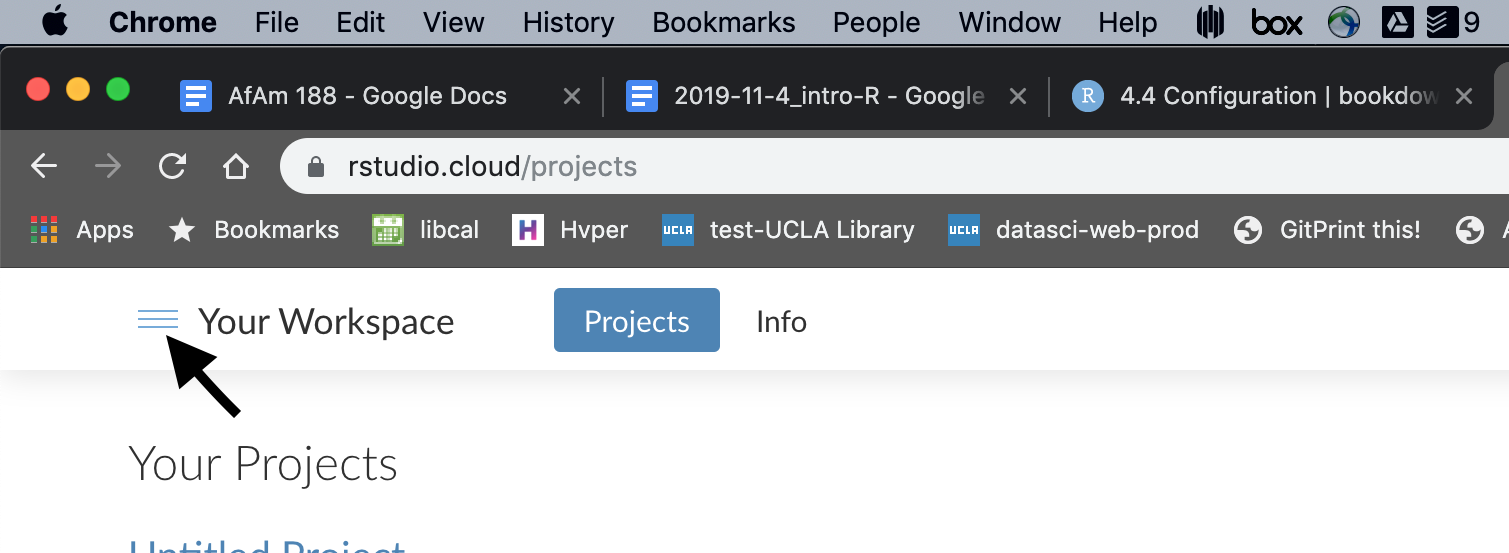
\includegraphics[width=0.9\linewidth]{images/rstudio-cloud}

Then select the Primers menu item:

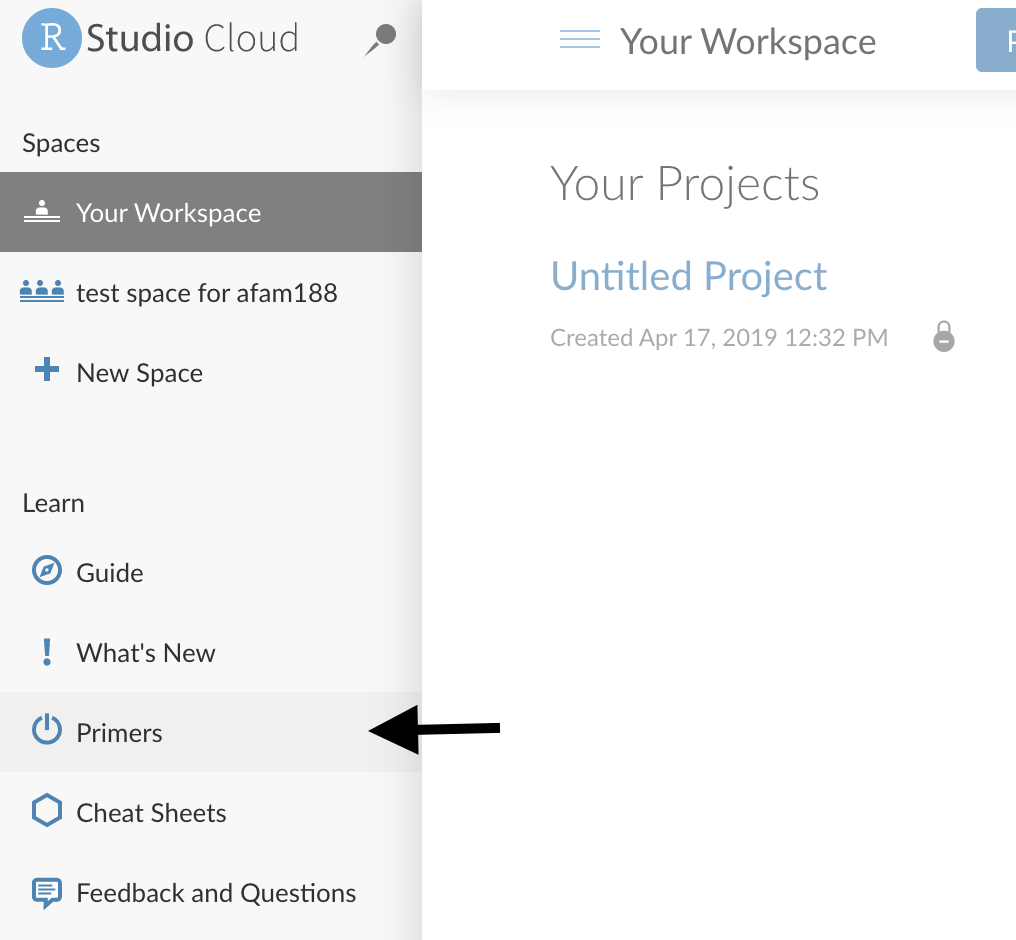
\includegraphics[width=0.9\linewidth]{images/primers}

Take the primer ``The Basics'', which has two tutorials named ``Visualization Basics'' and ``Programming Basics''. These will take you about between an 1.5 or 2.0 hours.

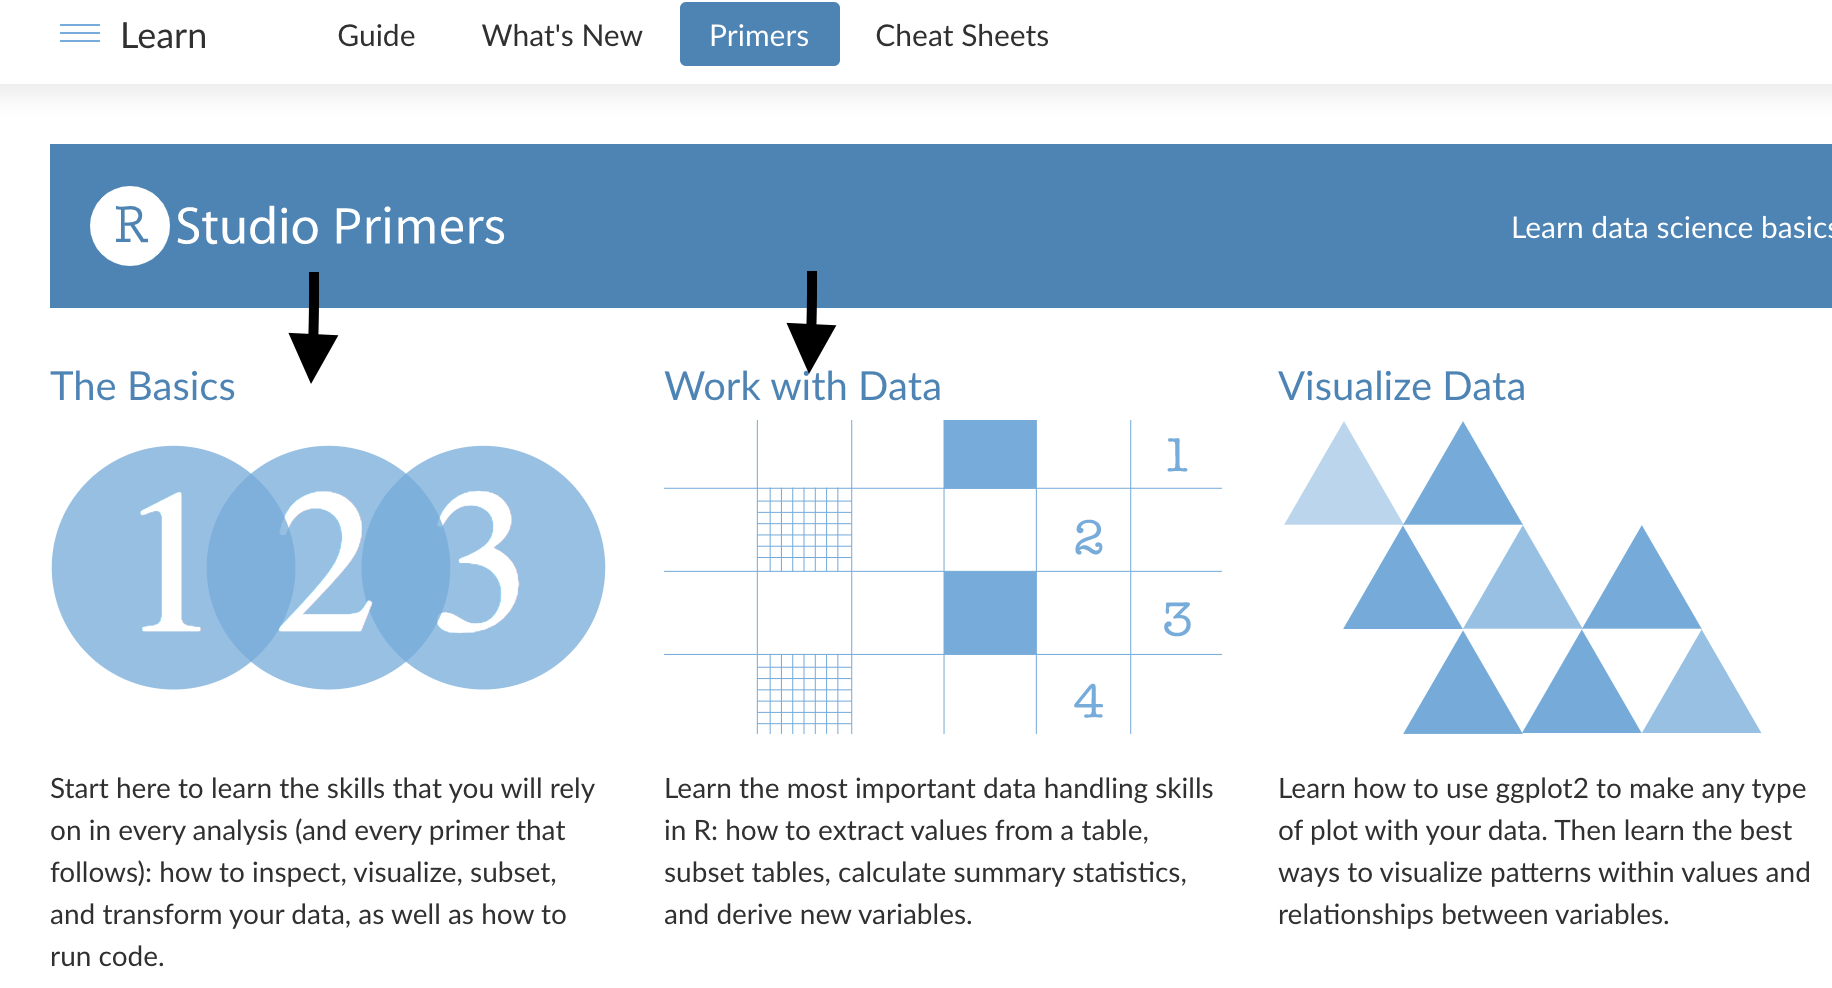
\includegraphics[width=400pt]{images/primers-todo}

\hypertarget{getting-started}{%
\chapter{Getting Started with Data in R}\label{getting-started}}

\hypertarget{learn-objectives}{%
\section{Learn Objectives}\label{learn-objectives}}

After this lesson, learners will be able to:

\begin{itemize}
\tightlist
\item
  Describe the purpose and use of each pane in the RStudio IDE
\item
  Locate buttons and options in the RStudio IDE
\item
  Know how to run code in R
\item
  How to save things to an object in R
\item
  Call functions
\item
  What packages are and where to install and load them
\item
  Inspecting data and doing simple plots
\item
  Make a map in R, exporting images in R
\end{itemize}

\hypertarget{r-RStudio}{%
\section{What are R and RStudio?}\label{r-RStudio}}

At its simplest, R is like a car's engine while RStudio is like a car's dashboard as illustrated in Figure.

\begin{figure}

{\centering 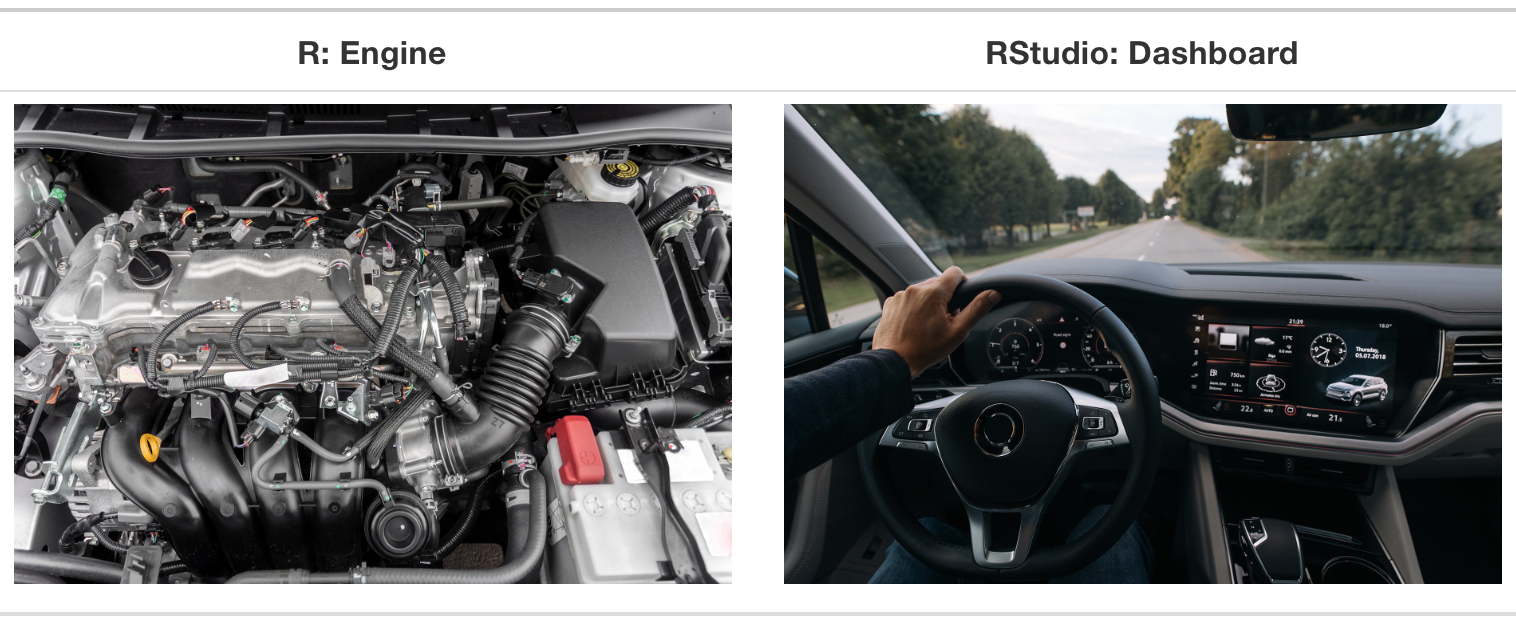
\includegraphics[width=0.95\linewidth]{images/shutterstock/R_vs_RStudio_1} 

}

\caption{Analogy of difference between R and RStudio.}\label{fig:R-vs-RStudio-1}
\end{figure}

More precisely, R is a \textbf{programming language} that runs computations, while RStudio is an \emph{integrated development environment (IDE)} that provides an interface by adding many convenient features and tools. So just as the way of having access to a speedometer, rearview mirrors, and a navigation system makes driving much easier, using RStudio's interface makes using R much easier as well.

\hypertarget{using-r-via-rstudio}{%
\subsection{Using R via RStudio}\label{using-r-via-rstudio}}

Recall our car analogy from earlier. Much as we don't drive a car by interacting directly with the engine but rather by interacting with elements on the car's dashboard, we won't be using R directly but rather we will use RStudio's interface.

\hypertarget{code}{%
\section{How do I code in R?}\label{code}}

Now that you're set up with R and RStudio in RStudio Cloud, you are probably asking yourself ``OK. Now how do I use R?''. The first thing to note is that unlike other statistical software \& mapping programs like Excel, SPSS, or QGIS that provide \href{https://en.wikipedia.org/wiki/Point_and_click}{point-and-click} interfaces, R is an \href{https://en.wikipedia.org/wiki/Interpreted_language}{interpreted language}. This means you have to type in commands written in \emph{R code}. In other words, you get to code/program in R. Note that we'll use the terms ``coding'' and ``programming'' interchangeably in this book.

While it is not required to be a seasoned coder/computer programmer to use R, there is still a set of basic programming concepts that R users need to understand. Consequently, while this class is not focused on programming, you will still learn just enough of these basic programming concepts needed to explore and analyze data effectively.

\hypertarget{programming-concepts}{%
\subsection{Basic programming concepts and terminology}\label{programming-concepts}}

We now introduce some basic programming concepts and terminology. Instead of asking you to learn all these concepts and terminology right now, we'll guide you so that you'll ``learn by doing.'' Note that in lesson we will always use a different font to distinguish regular text from \texttt{computer\_code}. The best way to master these topics is, in our opinions, through \href{https://jamesclear.com/deliberate-practice-theory}{deliberate practice} with R and lots of repetition.

\begin{itemize}
\tightlist
\item
  Basics: \index{programming language basics}

  \begin{itemize}
  \tightlist
  \item
    \emph{Console}: where you enter in commands. \index{console}
  \item
    \emph{Running code}: the act of telling R to perform an act by giving it commands in the console.
  \item
    \emph{Objects}: where values are saved in R. We'll show you how to \emph{assign} values to objects and how to display the contents of objects. \index{objects}
  \item
    \emph{Data types}: integers, doubles/numerics, logicals, and characters. \index{data types} Integers are values like -1, 0, 2, 4092. Doubles or numerics are a larger set of values containing both the integers but also fractions and decimal values like -24.932 and 0.8. Logicals are either \texttt{TRUE} or \texttt{FALSE} and characters are text such as ``cabbage'', ``The Wire'', and ``This ramen is delicious.'' Note that characters are often denoted with the quotation marks around them.
  \end{itemize}
\item
  \emph{Vectors}: a series of values. These are created using the \texttt{c()} function, where \texttt{c()} stands for ``combine'' or ``concatenate.'' For example, \texttt{c(6,\ 11,\ 13,\ 31,\ 90,\ 92)} creates a six element series of positive integer values \index{vectors}.
\item
  \emph{Factors}: \emph{categorical data} are commonly represented in R as factors. \index{factors} Categorical data can also be represented as \emph{strings}. We'll see this difference as we progress through the book.
\item
  \emph{Data frames}: rectangular spreadsheets. They are representations of datasets in R where the rows correspond to \emph{observations} and the columns correspond to \emph{variables} that describe the observations. \index{data frames} We'll cover data frames later in Section.
\item
  \emph{Conditionals}:

  \begin{itemize}
  \tightlist
  \item
    Testing for equality in R using \texttt{==} (and not \texttt{=}, which is typically used for assignment). For example, \texttt{2\ +\ 1\ ==\ 3} compares \texttt{2\ +\ 1} to \texttt{3} and is correct R code, while \texttt{2\ +\ 1\ =\ 3} will return an error.
  \item
    Boolean algebra: \texttt{TRUE/FALSE} statements and mathematical operators such as \texttt{\textless{}} (less than), \texttt{\textless{}=} (less than or equal), and \texttt{!=} (not equal to). \index{Boolean algebra} For example, \texttt{4\ +\ 2\ \textgreater{}=\ 3} will return \texttt{TRUE}, but \texttt{3\ +\ 5\ \textless{}=\ 1} will return \texttt{FALSE}.
  \item
    Logical operators: \texttt{\&} representing ``and'' as well as \texttt{\textbar{}} representing ``or.'' For example, \texttt{(2\ +\ 1\ ==\ 3)\ \&\ (2\ +\ 1\ ==\ 4)} returns \texttt{FALSE} since both clauses are not \texttt{TRUE} (only the first clause is \texttt{TRUE}). On the other hand, \texttt{(2\ +\ 1\ ==\ 3)\ \textbar{}\ (2\ +\ 1\ ==\ 4)} returns \texttt{TRUE} since at least one of the two clauses is \texttt{TRUE}.
  \end{itemize}
\item
  \emph{Functions}, also called \emph{commands}: Functions perform tasks in R. They take in inputs called \emph{arguments} and return outputs. You can either manually specify a function's arguments or use the function's \emph{default values}. \index{functions}

  \begin{itemize}
  \tightlist
  \item
    For example, the function \texttt{seq()} in R generates a sequence of numbers. If you just run \texttt{seq()} it will return the value 1. That doesn't seem very useful! This is because the default arguments are set as \texttt{seq(from\ =\ 1,\ to\ =\ 1)}. Thus, if you don't pass in different values for \texttt{from} and \texttt{to} to change this behavior, R just assumes all you want is the number 1. You can change the argument values by updating the values after the \texttt{=} sign. If we try out \texttt{seq(from\ =\ 2,\ to\ =\ 5)} we get the result \texttt{2\ 3\ 4\ 5} that we might expect.
  \item
    We'll work with functions a lot throughout this book and you'll get lots of practice in understanding their behaviors. To further assist you in understanding when a function is mentioned in the book, we'll also include the \texttt{()} after them as we did with \texttt{seq()} above.
  \end{itemize}
\end{itemize}

This list is by no means an exhaustive list of all the programming concepts and terminology needed to become a savvy R user; such a list would be so large it wouldn't be very useful, especially for novices. Rather, we feel this is a minimally viable list of programming concepts and terminology you need to know before getting started. We feel that you can learn the rest as you go. Remember that your mastery of all of these concepts and terminology will build as you practice more and more.

\hypertarget{messages}{%
\subsection{Errors, warnings, and messages}\label{messages}}

One thing that intimidates new R and RStudio users is how it reports \emph{errors}, \emph{warnings}, and \emph{messages}. R reports errors, warnings, and messages in a glaring red font, which makes it seem like it is scolding you. However, seeing red text in the console is not always bad.

R will show red text in the console pane in three different situations:

\begin{itemize}
\tightlist
\item
  \textbf{Errors}: When the red text is a legitimate error, it will be prefaced with ``Error in\ldots{}'' and will try to explain what went wrong. Generally when there's an error, the code will not run. For example, we'll see in Subsection if you see \texttt{Error\ in\ ggplot(...)\ :\ could\ not\ find\ function\ "ggplot"}, it means that the \texttt{ggplot()} function is not accessible because the package that contains the function (\texttt{ggplot2}) was not loaded with \texttt{library(ggplot2)}. Thus you cannot use the \texttt{ggplot()} function without the \texttt{ggplot2} package being loaded first.
\item
  \textbf{Warnings}: When the red text is a warning, it will be prefaced with ``Warning:'' and R will try to explain why there's a warning. Generally your code will still work, but with some caveats.\\
\item
  \textbf{Messages}: When the red text doesn't start with either ``Error'' or ``Warning'', it's \emph{just a friendly message}. You'll see these messages when you load \emph{R packages} in the upcoming Subsection or when you read data saved in spreadsheet files with the \texttt{read\_csv()} function. These are helpful diagnostic messages and they don't stop your code from working. Additionally, you'll see these messages when you install packages too using \texttt{install.packages()}.
\end{itemize}

Remember, when you see red text in the console, \emph{don't panic}. It doesn't necessarily mean anything is wrong. Rather:

\begin{itemize}
\tightlist
\item
  If the text starts with ``Error'', figure out what's causing it. {Think of errors as a red traffic light: something is wrong!}
\item
  If the text starts with ``Warning'', figure out if it's something to worry about. For instance, if you get a warning about missing values in a scatterplot and you know there are missing values, you're fine. If that's surprising, look at your data and see what's missing. {Think of warnings as a yellow traffic light: everything is working fine, but watch out/pay attention.}
\item
  Otherwise, the text is just a message. Read it, wave back at R, and thank it for talking to you. {Think of messages as a green traffic light: everything is working fine and keep on going!}
\end{itemize}

\hypertarget{tips-code}{%
\subsection{Tips on learning to code}\label{tips-code}}

Learning to code/program is quite similar to learning a foreign language. It can be daunting and frustrating at first. Such frustrations are common and it is normal to feel discouraged as you learn. However, just as with learning a foreign language, if you put in the effort and are not afraid to make mistakes, anybody can learn and improve.

Here are a few useful tips to keep in mind as you learn to program:

\begin{itemize}
\tightlist
\item
  \textbf{Remember that computers are not actually that smart}: You may think your computer or smartphone is ``smart,'' but really people spent a lot of time and energy designing them to appear ``smart.'' In reality, you have to tell a computer everything it needs to do. Furthermore, the instructions you give your computer can't have any mistakes in them, nor can they be ambiguous in any way.
\item
  \textbf{Take the ``copy, paste, and tweak'' approach}: Especially when you learn your first programming language or you need to understand particularly complicated code, it is often much easier to take existing code that you know works and modify it to suit your ends. This is as opposed to trying to type out the code from scratch. We call this the \emph{``copy, paste, and tweak''} approach. So early on, we suggest not trying to write code from memory, but rather take existing examples we have provided you, then copy, paste, and tweak them to suit your goals. After you start feeling more confident, you can slowly move away from this approach. Think of the ``copy, paste, and tweak'' approach as training wheels for a child learning to ride a bike. After getting comfortable, they won't need them anymore.
\item
  \textbf{The best way to learn to code is by doing}: Rather than learning to code for its own sake, we find that learning to code goes much smoother when you have a goal in mind or when you are working on a particular project, like analyzing data that you are interested in and that is important to you.
\item
  \textbf{Practice is key}: Just as the only method to improve your foreign language skills is through lots of practice and speaking, the only method to improving your coding skills is through lots of practice. Don't worry, however, we'll give you plenty of opportunities to do so!
\end{itemize}

\hypertarget{how-to-run-codefirst-script}{%
\section{How to run code/first script}\label{how-to-run-codefirst-script}}

\begin{itemize}
\tightlist
\item
  We can do basic math in R
\item
  To run the code we can put our cursor on the line we want to run and click on Run in the top right of the script pane.
\item
  We can also highlight multiple lines of code and click Run
\item
  This is good, but it takes extra time to click and point when you are coding, so RStudio have keyboard shortcuts to let you run code.
\item
  Use + on Mac and + on windows
\item
  let's try a few more expressions:
\end{itemize}

\begin{Shaded}
\begin{Highlighting}[]
\CommentTok{#a string or character sequence is like a name or sentence or alpha numberic in R}
\StringTok{"Tim Dennis"}
\end{Highlighting}
\end{Shaded}

\begin{verbatim}
## [1] "Tim Dennis"
\end{verbatim}

\begin{Shaded}
\begin{Highlighting}[]
\CommentTok{# we can use arithmetic on strings}
\StringTok{"Your Name"}
\end{Highlighting}
\end{Shaded}

\begin{verbatim}
## [1] "Your Name"
\end{verbatim}

\hypertarget{arrests}{%
\section{Explore your first datasets}\label{arrests}}

The data we'll use is in our \texttt{data/} folder. Let's look at it - its a CSV? What does that stand for?

Data comes to us in a variety of formats, from pictures to text to numbers. Throughout this class, we'll focus on datasets that are saved in ``spreadsheet''-type format. This is probably the most common way data are collected and saved in many fields. But in R, we can read in data in many formats - this means that R will load the data into it's environment and make it ready for R to work with it.

Before we start exploring our \texttt{arrests} data in R, let's first load the packages needed for this lesson. What's a package? We haven't talked about those yet?

\hypertarget{what-are-packages}{%
\section{What are Packages}\label{what-are-packages}}

R packages extend the functionality of R by providing additional functions, data, and documentation. They are written by a worldwide community of R users and can be downloaded for free from the internet.

A good analogy for R packages is they are like apps you can download onto a mobile phone:

\begin{figure}

{\centering 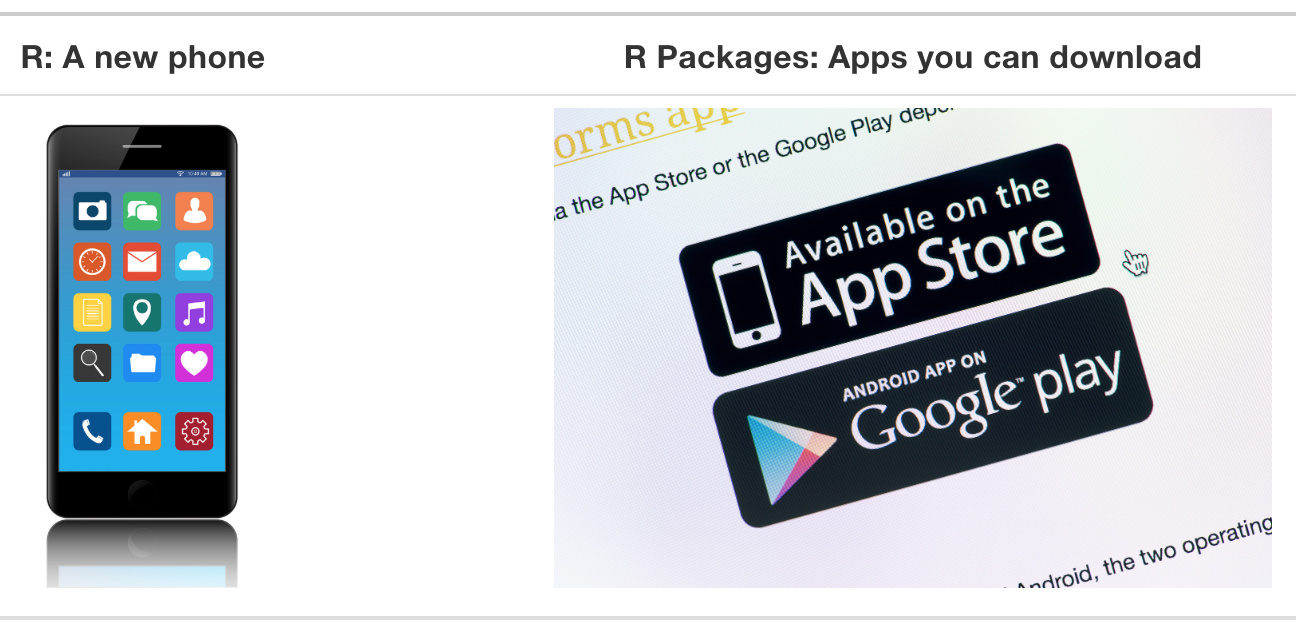
\includegraphics[width=0.7\linewidth]{images/shutterstock/R_vs_R_packages} 

}

\caption{Analogy of R versus R packages.}\label{fig:R-vs-R-packages}
\end{figure}

So R is like a new mobile phone: while it has a certain amount of features when you use it for the first time, it doesn't have everything. R packages are like the apps you can download onto your phone from Apple's App Store or Android's Google Play.

What are the steps to doing this? To install a package, click on the Packages tab on the right bottom pane. Now you can click \textbf{Install} and start typing the package you want to install and it will download.

How do you find out about packages? Take a look at \href{https://cran.r-project.org/web/views/}{task views} on the CRAN (Comprehensive R Archive Network). Packages are grouped by topic. For this class, because we are using R Studio Cloud, I've already installed the packages we need.

Once you install a package you need to tell R you want to use it. We do this with the \texttt{library()} function. Ok but what is a function? Anybody know? Right functions perform tasks in R. They take inputs called \textbf{arguments} (in this case our csv file) and return some kind of output. \texttt{library()} takes a package we want to use in our R code and loads it into our current R environment. Let's try now:

\begin{Shaded}
\begin{Highlighting}[]
\KeywordTok{library}\NormalTok{(tidyverse)}
\end{Highlighting}
\end{Shaded}

\texttt{tidyverse} gives us access to a bunch of other functions we can now use after it is loaded. One is called \texttt{read\_csv()}. What if we know we need to use \texttt{read\_csv()} to read in our data, but we don't know how. What would we do? We use R's built in help features to get information on the functions. In R we use a \texttt{?} before the function without the trailing parentheses. Type this code in RStudio and run it:

\begin{Shaded}
\begin{Highlighting}[]
\NormalTok{?read_csv}
\end{Highlighting}
\end{Shaded}

It opens the help documentation in the \textbf{Help} tab in the bottom right RStudio pane. It contains a description, usage, arguments and at the bottom, examples, for the function. We see the first argument of \texttt{read\_csv()} is a \textbf{file} meaning \texttt{read\_csv()} needs the file location so it can read the file into R. With this information let's read write our \texttt{read\_csv()} function so it knows where our arrests data is. Remember from earlier, the arrests data is in the \texttt{data/} folder in our project.

Run the the following code:

\begin{Shaded}
\begin{Highlighting}[]
\KeywordTok{read_csv}\NormalTok{(}\StringTok{'data/aug6_12_arrest_data.csv'}\NormalTok{)}
\end{Highlighting}
\end{Shaded}

Ok, notice we need to quote the file location and name. This is because files paths and names are strings in R. Now when we run it, it outputs the dataset to the console. That's great! We can see our data. Let's get practice running it by running it again.

\begin{Shaded}
\begin{Highlighting}[]
\KeywordTok{read_csv}\NormalTok{(}\StringTok{'data/aug6_12_arrest_data.csv'}\NormalTok{)}
\end{Highlighting}
\end{Shaded}

\begin{verbatim}
## Parsed with column specification:
## cols(
##   latitude = col_double(),
##   longitude = col_double(),
##   zipcode = col_double(),
##   arr_date2 = col_date(format = ""),
##   arrest_time = col_time(format = ""),
##   age = col_double(),
##   sex = col_character(),
##   race_cat = col_character(),
##   arrest_type = col_character(),
##   charge = col_character()
## )
\end{verbatim}

\begin{verbatim}
## # A tibble: 2,368 x 10
##    latitude longitude zipcode arr_date2  arrest_time   age sex   race_cat
##       <dbl>     <dbl>   <dbl> <date>     <time>      <dbl> <chr> <chr>   
##  1     34.0     -118.   90021 2018-08-12 15:00          52 M     LatinX  
##  2     33.9     -118.   90059 2018-08-12 22:00          37 M     Black   
##  3     34.1     -118.   90036 2018-08-12 22:20          28 M     Black   
##  4     34.2     -118.   91605 2018-08-12 18:40          28 M     LatinX  
##  5     34.0     -118.   90037 2018-08-12 19:30          23 M     LatinX  
##  6     34.3     -118.   91342 2018-08-12 19:48          36 M     LatinX  
##  7     34.2     -119.   91324 2018-08-12 01:35          62 M     LatinX  
##  8     34.2     -118.   91401 2018-08-12 15:00          36 M     Other   
##  9     34.1     -118.   90046 2018-08-12 15:00          28 M     Black   
## 10     34.1     -118.   91604 2018-08-12 08:00          53 M     White   
## # ... with 2,358 more rows, and 2 more variables: arrest_type <chr>,
## #   charge <chr>
\end{verbatim}

Look at the output in the console. It gives us some important information about our data frame.

\begin{challenge}
\hypertarget{inspect-the-console-data-output}{%
\subsection{Inspect the Console Data
Output}\label{inspect-the-console-data-output}}

What does the output tell us? How many rows are in our data? Columns?
What about this part?

\begin{quote}
cols( latitude = col\_double(),\\
longitude = col\_double(),\\
zipcode = col\_double(),\\
age = col\_double(),\\
sex = col\_character(),\\
race\_cat = col\_character(),\\
arrest\_type = col\_character(),\\
arr\_date2 = col\_date(format = "")\\
)
\end{quote}

What is this telling us about our data?
\end{challenge}

Yes, the last part tells us the type of data R thinks our data is. \texttt{age} is a number of double type, \texttt{sex} is a character type, \texttt{arr\_date2} is a date.

This has been helpful, but the problem is we want to do more with our data than outputting it to the console. In order to save our data and work on it, we need to make it into an object in R. Let's do this now by typing the following and running it:

\begin{Shaded}
\begin{Highlighting}[]
\NormalTok{arrests <-}\StringTok{ }\KeywordTok{read_csv}\NormalTok{(}\StringTok{'data/aug6_12_arrest_data.csv'}\NormalTok{)}
\end{Highlighting}
\end{Shaded}

\begin{verbatim}
## Parsed with column specification:
## cols(
##   latitude = col_double(),
##   longitude = col_double(),
##   zipcode = col_double(),
##   arr_date2 = col_date(format = ""),
##   arrest_time = col_time(format = ""),
##   age = col_double(),
##   sex = col_character(),
##   race_cat = col_character(),
##   arrest_type = col_character(),
##   charge = col_character()
## )
\end{verbatim}

\begin{callout}
\hypertarget{getting-data-into-rstudio-cloud}{%
\subsection{Getting data into RStudio
Cloud}\label{getting-data-into-rstudio-cloud}}

The data we are using in this class has been provided for us, but what
if you want to get data into RStudio Cloud?
\end{callout}

\hypertarget{what-to-do-first-after-you-read-in-your-data}{%
\section{What to do first after you read in your data?}\label{what-to-do-first-after-you-read-in-your-data}}

After we run this, notice the top left \textbf{Environment} tab in RStudio. We now see \texttt{arrests} listed under \textbf{Data}. We can click on that to open and look at it in an \texttt{arrests} tab in our main editing window. Take a moment and explore the data via this window? Notice you can filter the data, sort and view the data, but not edit it.

The below functions take as their ``argument'' (their input) the data frame.

\begin{enumerate}
\def\labelenumi{\arabic{enumi}.}
\tightlist
\item
  Using the \texttt{View()} function, which brings up RStudio's built-in spreadsheet viewer.
\end{enumerate}

\begin{itemize}
\tightlist
\item
  This is the same as clicking on the data frame in the \textbf{Environment} tab
\end{itemize}

\begin{enumerate}
\def\labelenumi{\arabic{enumi}.}
\tightlist
\item
  Using the \texttt{glimpse()} function, which is included in the \texttt{dplyr} package.
\item
  Using the \texttt{str()} function - gives you similar info as \texttt{glimpse()}
\item
  The functions \texttt{head()} and \texttt{tail()} also let you inspect the data frame.
\item
  \texttt{\$} is a symbol that let's us look at one column of a data frame, like so:
\end{enumerate}

\begin{Shaded}
\begin{Highlighting}[]
\NormalTok{arrests}\OperatorTok{$}\NormalTok{race_cat}
\end{Highlighting}
\end{Shaded}

\begin{verbatim}
##    [1] "LatinX" "Black"  "Black"  "LatinX" "LatinX" "LatinX" "LatinX"
##    [8] "Other"  "Black"  "White"  "White"  "White"  "LatinX" "White" 
##   [15] "LatinX" "LatinX" "LatinX" "White"  "LatinX" "Black"  "LatinX"
##   [22] "LatinX" "Other"  "LatinX" "LatinX" "White"  "LatinX" "LatinX"
##   [29] "Other"  "LatinX" "LatinX" "LatinX" "Black"  "White"  "Black" 
##   [36] "Other"  "White"  "Black"  "Black"  "Black"  "White"  "White" 
##   [43] "LatinX" "Black"  "White"  "Black"  "Black"  "LatinX" "LatinX"
##   [50] "Other"  "Black"  "LatinX" "LatinX" "LatinX" "LatinX" "Black" 
##   [57] "White"  "LatinX" "LatinX" "LatinX" "LatinX" "LatinX" "Other" 
##   [64] "White"  "LatinX" "White"  "Black"  "Other"  "White"  "LatinX"
##   [71] "LatinX" "White"  "White"  "LatinX" "LatinX" "LatinX" "Black" 
##   [78] "LatinX" "LatinX" "LatinX" "LatinX" "LatinX" "LatinX" "White" 
##   [85] "LatinX" "LatinX" "LatinX" "Black"  "Black"  "LatinX" "LatinX"
##   [92] "White"  "Black"  "LatinX" "LatinX" "White"  "LatinX" "LatinX"
##   [99] "LatinX" "LatinX" "LatinX" "LatinX" "LatinX" "LatinX" "LatinX"
##  [106] "Black"  "LatinX" "LatinX" "Other"  "LatinX" "LatinX" "LatinX"
##  [113] "White"  "Black"  "White"  "White"  "White"  "LatinX" "LatinX"
##  [120] "Black"  "White"  "LatinX" "Other"  "LatinX" "Black"  "LatinX"
##  [127] "LatinX" "Black"  "White"  "LatinX" "Black"  "LatinX" "LatinX"
##  [134] "LatinX" "Black"  "White"  "LatinX" "Black"  "White"  "LatinX"
##  [141] "LatinX" "Black"  "LatinX" "Black"  "White"  "Black"  "LatinX"
##  [148] "LatinX" "LatinX" "LatinX" "White"  "LatinX" "LatinX" "Black" 
##  [155] "LatinX" "LatinX" "Black"  "White"  "Other"  "LatinX" "LatinX"
##  [162] "Other"  "LatinX" "LatinX" "LatinX" "Black"  "Other"  "LatinX"
##  [169] "LatinX" "White"  "LatinX" "LatinX" "Black"  "Black"  "LatinX"
##  [176] "White"  "Black"  "Other"  "LatinX" "LatinX" "LatinX" "Black" 
##  [183] "White"  "White"  "LatinX" "Black"  "LatinX" "LatinX" "LatinX"
##  [190] "Black"  "LatinX" "LatinX" "LatinX" "LatinX" "LatinX" "LatinX"
##  [197] "Black"  "Black"  "LatinX" "Black"  "Black"  "Black"  "Black" 
##  [204] "LatinX" "Black"  "Black"  "LatinX" "Black"  "LatinX" "Black" 
##  [211] "Black"  "LatinX" "White"  "Black"  "LatinX" "LatinX" "LatinX"
##  [218] "Black"  "LatinX" "White"  "White"  "LatinX" "White"  "LatinX"
##  [225] "LatinX" "LatinX" "LatinX" "LatinX" "LatinX" "LatinX" "LatinX"
##  [232] "Black"  "Black"  "LatinX" "LatinX" "Black"  "LatinX" "Black" 
##  [239] "LatinX" "LatinX" "LatinX" "Black"  "LatinX" "Black"  "LatinX"
##  [246] "White"  "LatinX" "LatinX" "LatinX" "LatinX" "LatinX" "Black" 
##  [253] "Black"  "White"  "Black"  "LatinX" "LatinX" "White"  "LatinX"
##  [260] "LatinX" "LatinX" "LatinX" "LatinX" "LatinX" "LatinX" "Other" 
##  [267] "Black"  "LatinX" "LatinX" "White"  "White"  "Other"  "LatinX"
##  [274] "White"  "White"  "LatinX" "Black"  "LatinX" "LatinX" "Black" 
##  [281] "White"  "LatinX" "White"  "LatinX" "LatinX" "Black"  "LatinX"
##  [288] "Black"  "LatinX" "Black"  "White"  "White"  "LatinX" "Black" 
##  [295] "Black"  "LatinX" "Black"  "LatinX" "LatinX" "LatinX" "LatinX"
##  [302] "LatinX" "LatinX" "Black"  "White"  "LatinX" "Black"  "Black" 
##  [309] "Black"  "LatinX" "White"  "LatinX" "White"  "LatinX" "Black" 
##  [316] "LatinX" "LatinX" "LatinX" "LatinX" "LatinX" "Black"  "White" 
##  [323] "White"  "Black"  "Black"  "White"  "LatinX" "Black"  "LatinX"
##  [330] "LatinX" "Black"  "LatinX" "Black"  "Black"  "LatinX" "White" 
##  [337] "Black"  "LatinX" "LatinX" "Black"  "Black"  "Black"  "LatinX"
##  [344] "Black"  "Black"  "LatinX" "LatinX" "LatinX" "LatinX" "LatinX"
##  [351] "White"  "LatinX" "White"  "LatinX" "LatinX" "LatinX" "LatinX"
##  [358] "White"  "Black"  "Black"  "White"  "White"  "White"  "LatinX"
##  [365] "LatinX" "LatinX" "LatinX" "Black"  "LatinX" "Black"  "LatinX"
##  [372] "Black"  "LatinX" "Black"  "LatinX" "LatinX" "Other"  "LatinX"
##  [379] "Black"  "Black"  "LatinX" "LatinX" "LatinX" "LatinX" "LatinX"
##  [386] "Black"  "White"  "Black"  "Black"  "LatinX" "Black"  "LatinX"
##  [393] "LatinX" "Black"  "White"  "Black"  "White"  "Black"  "LatinX"
##  [400] "Black"  "Black"  "LatinX" "Black"  "Black"  "Black"  "Black" 
##  [407] "Black"  "White"  "White"  "LatinX" "White"  "LatinX" "LatinX"
##  [414] "LatinX" "LatinX" "LatinX" "Other"  "LatinX" "LatinX" "Black" 
##  [421] "Black"  "LatinX" "Black"  "Black"  "Black"  "Other"  "LatinX"
##  [428] "Black"  "LatinX" "LatinX" "LatinX" "LatinX" "Black"  "Black" 
##  [435] "LatinX" "LatinX" "Black"  "LatinX" "Black"  "Black"  "LatinX"
##  [442] "LatinX" "Black"  "Black"  "LatinX" "LatinX" "LatinX" "Other" 
##  [449] "Black"  "LatinX" "LatinX" "Other"  "LatinX" "LatinX" "Black" 
##  [456] "Black"  "LatinX" "LatinX" "LatinX" "White"  "LatinX" "White" 
##  [463] "LatinX" "Other"  "LatinX" "LatinX" "Black"  "LatinX" "White" 
##  [470] "Black"  "White"  "LatinX" "Other"  "LatinX" "Black"  "White" 
##  [477] "Black"  "LatinX" "White"  "White"  "LatinX" "LatinX" "LatinX"
##  [484] "LatinX" "LatinX" "LatinX" "Black"  "LatinX" "LatinX" "LatinX"
##  [491] "LatinX" "LatinX" "LatinX" "White"  "Black"  "Black"  "Black" 
##  [498] "LatinX" "LatinX" "LatinX" "Black"  "LatinX" "LatinX" "Black" 
##  [505] "Black"  "LatinX" "LatinX" "White"  "LatinX" "Black"  "White" 
##  [512] "Black"  "LatinX" "White"  "White"  "LatinX" "Black"  "LatinX"
##  [519] "White"  "LatinX" "Black"  "LatinX" "LatinX" "LatinX" "LatinX"
##  [526] "White"  "LatinX" "LatinX" "LatinX" "LatinX" "Black"  "LatinX"
##  [533] "LatinX" "Black"  "Black"  "Black"  "White"  "White"  "LatinX"
##  [540] "Other"  "White"  "LatinX" "Black"  "LatinX" "LatinX" "LatinX"
##  [547] "White"  "LatinX" "LatinX" "LatinX" "LatinX" "White"  "LatinX"
##  [554] "Black"  "LatinX" "Black"  "Black"  "Other"  "LatinX" "Other" 
##  [561] "LatinX" "White"  "Other"  "LatinX" "LatinX" "LatinX" "Black" 
##  [568] "LatinX" "Other"  "Black"  "LatinX" "Black"  "LatinX" "LatinX"
##  [575] "LatinX" "LatinX" "Other"  "LatinX" "Black"  "Other"  "LatinX"
##  [582] "Other"  "LatinX" "LatinX" "White"  "LatinX" "LatinX" "LatinX"
##  [589] "LatinX" "White"  "LatinX" "Black"  "LatinX" "Black"  "Black" 
##  [596] "LatinX" "Other"  "LatinX" "LatinX" "LatinX" "Other"  "LatinX"
##  [603] "LatinX" "White"  "LatinX" "Black"  "White"  "Black"  "Other" 
##  [610] "LatinX" "LatinX" "Black"  "White"  "Black"  "Black"  "LatinX"
##  [617] "LatinX" "LatinX" "LatinX" "Other"  "White"  "White"  "LatinX"
##  [624] "Black"  "White"  "Black"  "LatinX" "White"  "Black"  "LatinX"
##  [631] "Other"  "White"  "White"  "White"  "LatinX" "LatinX" "Black" 
##  [638] "LatinX" "LatinX" "LatinX" "White"  "LatinX" "Black"  "LatinX"
##  [645] "Other"  "Black"  "Black"  "White"  "Other"  "LatinX" "LatinX"
##  [652] "Black"  "LatinX" "Black"  "Other"  "Black"  "LatinX" "White" 
##  [659] "White"  "White"  "Black"  "LatinX" "White"  "Black"  "LatinX"
##  [666] "LatinX" "LatinX" "LatinX" "White"  "Black"  "Black"  "LatinX"
##  [673] "White"  "LatinX" "LatinX" "Black"  "LatinX" "LatinX" "White" 
##  [680] "LatinX" "LatinX" "Black"  "Black"  "Black"  "Other"  "White" 
##  [687] "LatinX" "White"  "LatinX" "LatinX" "Black"  "Black"  "LatinX"
##  [694] "Black"  "Black"  "Black"  "Black"  "Black"  "White"  "White" 
##  [701] "LatinX" "LatinX" "White"  "White"  "LatinX" "LatinX" "Black" 
##  [708] "LatinX" "LatinX" "LatinX" "Other"  "Black"  "White"  "White" 
##  [715] "Black"  "Other"  "Black"  "LatinX" "LatinX" "LatinX" "LatinX"
##  [722] "Black"  "Black"  "Black"  "White"  "LatinX" "LatinX" "White" 
##  [729] "LatinX" "LatinX" "White"  "LatinX" "White"  "White"  "Black" 
##  [736] "LatinX" "Black"  "Black"  "LatinX" "LatinX" "LatinX" "White" 
##  [743] "LatinX" "Black"  "LatinX" "LatinX" "Black"  "White"  "LatinX"
##  [750] "Black"  "Black"  "Black"  "LatinX" "White"  "LatinX" "White" 
##  [757] "LatinX" "White"  "LatinX" "White"  "LatinX" "Black"  "White" 
##  [764] "Black"  "LatinX" "Black"  "Black"  "White"  "Black"  "Black" 
##  [771] "LatinX" "White"  "LatinX" "Black"  "Black"  "White"  "White" 
##  [778] "White"  "LatinX" "Other"  "LatinX" "White"  "White"  "LatinX"
##  [785] "LatinX" "LatinX" "White"  "Black"  "Black"  "White"  "Black" 
##  [792] "White"  "LatinX" "LatinX" "LatinX" "LatinX" "LatinX" "LatinX"
##  [799] "Black"  "Black"  "LatinX" "Black"  "LatinX" "LatinX" "Black" 
##  [806] "White"  "Other"  "LatinX" "LatinX" "White"  "Other"  "LatinX"
##  [813] "White"  "Other"  "LatinX" "White"  "White"  "LatinX" "LatinX"
##  [820] "White"  "LatinX" "White"  "Black"  "LatinX" "LatinX" "White" 
##  [827] "White"  "LatinX" "LatinX" "White"  "Other"  "LatinX" "Black" 
##  [834] "Black"  "Black"  "LatinX" "LatinX" "LatinX" "Black"  "White" 
##  [841] "Black"  "Black"  "LatinX" "LatinX" "Black"  "LatinX" "White" 
##  [848] "LatinX" "LatinX" "LatinX" "White"  "White"  "White"  "White" 
##  [855] "LatinX" "Black"  "White"  "LatinX" "LatinX" "White"  "Black" 
##  [862] "White"  "Black"  "LatinX" "Black"  "LatinX" "LatinX" "LatinX"
##  [869] "Black"  "White"  "White"  "Black"  "LatinX" "White"  "White" 
##  [876] "Black"  "LatinX" "Black"  "White"  "Black"  "White"  "Black" 
##  [883] "White"  "LatinX" "LatinX" "Black"  "LatinX" "Black"  "White" 
##  [890] "LatinX" "White"  "White"  "LatinX" "White"  "LatinX" "LatinX"
##  [897] "LatinX" "Black"  "Black"  "White"  "Black"  "LatinX" "LatinX"
##  [904] "White"  "LatinX" "White"  "Black"  "LatinX" "Black"  "Black" 
##  [911] "Other"  "White"  "LatinX" "White"  "LatinX" "Black"  "LatinX"
##  [918] "LatinX" "LatinX" "Black"  "LatinX" "Black"  "LatinX" "LatinX"
##  [925] "White"  "Black"  "White"  "Other"  "Other"  "Black"  "LatinX"
##  [932] "Black"  "Other"  "LatinX" "LatinX" "Black"  "LatinX" "LatinX"
##  [939] "Other"  "Black"  "LatinX" "LatinX" "LatinX" "White"  "LatinX"
##  [946] "Black"  "White"  "LatinX" "LatinX" "Black"  "Black"  "White" 
##  [953] "Black"  "LatinX" "LatinX" "Black"  "White"  "LatinX" "LatinX"
##  [960] "LatinX" "LatinX" "LatinX" "LatinX" "Black"  "Black"  "Black" 
##  [967] "LatinX" "Other"  "Black"  "Black"  "LatinX" "Black"  "Black" 
##  [974] "White"  "Black"  "White"  "Black"  "Black"  "Black"  "Black" 
##  [981] "Black"  "Black"  "Other"  "LatinX" "LatinX" "Other"  "LatinX"
##  [988] "LatinX" "Black"  "White"  "LatinX" "Black"  "Black"  "Other" 
##  [995] "LatinX" "Black"  "LatinX" "LatinX" "White"  "LatinX" "Black" 
## [1002] "Black"  "LatinX" "Black"  "Black"  "White"  "Black"  "Other" 
## [1009] "Black"  "White"  "LatinX" "Other"  "LatinX" "LatinX" "LatinX"
## [1016] "Other"  "LatinX" "Black"  "LatinX" "Black"  "LatinX" "LatinX"
## [1023] "LatinX" "LatinX" "LatinX" "Black"  "Other"  "Other"  "White" 
## [1030] "LatinX" "Other"  "White"  "LatinX" "LatinX" "White"  "LatinX"
## [1037] "Black"  "Other"  "LatinX" "White"  "White"  "LatinX" "White" 
## [1044] "LatinX" "Black"  "White"  "White"  "Black"  "LatinX" "Black" 
## [1051] "LatinX" "LatinX" "White"  "LatinX" "Black"  "Other"  "LatinX"
## [1058] "Other"  "Black"  "White"  "Black"  "Black"  "Black"  "LatinX"
## [1065] "LatinX" "Black"  "Other"  "White"  "Black"  "White"  "White" 
## [1072] "White"  "Black"  "White"  "LatinX" "Black"  "LatinX" "White" 
## [1079] "LatinX" "Black"  "LatinX" "Black"  "White"  "Black"  "LatinX"
## [1086] "White"  "White"  "Other"  "Black"  "Other"  "LatinX" "LatinX"
## [1093] "LatinX" "LatinX" "Black"  "Black"  "White"  "LatinX" "Black" 
## [1100] "LatinX" "White"  "Black"  "LatinX" "LatinX" "LatinX" "White" 
## [1107] "LatinX" "LatinX" "LatinX" "LatinX" "LatinX" "LatinX" "Black" 
## [1114] "Black"  "LatinX" "LatinX" "LatinX" "Black"  "Black"  "Black" 
## [1121] "LatinX" "Black"  "Black"  "LatinX" "Black"  "LatinX" "White" 
## [1128] "Black"  "Black"  "Black"  "Black"  "LatinX" "Black"  "LatinX"
## [1135] "LatinX" "LatinX" "LatinX" "LatinX" "LatinX" "Black"  "LatinX"
## [1142] "Black"  "LatinX" "LatinX" "White"  "Other"  "White"  "LatinX"
## [1149] "White"  "White"  "LatinX" "Black"  "White"  "LatinX" "Black" 
## [1156] "LatinX" "Black"  "White"  "Other"  "White"  "Black"  "Black" 
## [1163] "White"  "Black"  "LatinX" "Black"  "LatinX" "Black"  "Other" 
## [1170] "Other"  "LatinX" "Black"  "Black"  "Black"  "White"  "White" 
## [1177] "LatinX" "Black"  "White"  "LatinX" "Black"  "LatinX" "Other" 
## [1184] "LatinX" "LatinX" "White"  "Black"  "White"  "LatinX" "White" 
## [1191] "LatinX" "Black"  "White"  "LatinX" "White"  "Black"  "White" 
## [1198] "LatinX" "LatinX" "Black"  "White"  "Black"  "Other"  "White" 
## [1205] "LatinX" "White"  "Black"  "White"  "Black"  "LatinX" "Black" 
## [1212] "LatinX" "Black"  "LatinX" "Black"  "LatinX" "LatinX" "White" 
## [1219] "LatinX" "LatinX" "White"  "LatinX" "LatinX" "LatinX" "Black" 
## [1226] "Black"  "Other"  "White"  "Black"  "White"  "Black"  "LatinX"
## [1233] "LatinX" "Other"  "LatinX" "White"  "White"  "Black"  "Black" 
## [1240] "LatinX" "LatinX" "White"  "LatinX" "LatinX" "LatinX" "LatinX"
## [1247] "LatinX" "Other"  "Black"  "White"  "LatinX" "LatinX" "White" 
## [1254] "LatinX" "LatinX" "LatinX" "LatinX" "LatinX" "LatinX" "Black" 
## [1261] "Black"  "LatinX" "Other"  "Other"  "LatinX" "Black"  "LatinX"
## [1268] "LatinX" "Black"  "LatinX" "Black"  "Black"  "LatinX" "LatinX"
## [1275] "LatinX" "LatinX" "LatinX" "LatinX" "Black"  "White"  "Black" 
## [1282] "LatinX" "White"  "LatinX" "Other"  "Black"  "LatinX" "Black" 
## [1289] "LatinX" "LatinX" "LatinX" "Black"  "White"  "White"  "LatinX"
## [1296] "LatinX" "Black"  "LatinX" "LatinX" "LatinX" "Black"  "Other" 
## [1303] "LatinX" "Other"  "Black"  "LatinX" "Black"  "LatinX" "Other" 
## [1310] "Black"  "Black"  "Black"  "LatinX" "LatinX" "Black"  "White" 
## [1317] "Other"  "LatinX" "LatinX" "LatinX" "LatinX" "Black"  "White" 
## [1324] "Black"  "White"  "Black"  "Black"  "LatinX" "Other"  "White" 
## [1331] "LatinX" "LatinX" "LatinX" "LatinX" "Black"  "Black"  "LatinX"
## [1338] "White"  "LatinX" "LatinX" "Other"  "Other"  "Black"  "Black" 
## [1345] "LatinX" "Black"  "Black"  "LatinX" "White"  "LatinX" "LatinX"
## [1352] "White"  "LatinX" "LatinX" "LatinX" "White"  "Black"  "LatinX"
## [1359] "LatinX" "Black"  "LatinX" "Black"  "LatinX" "Black"  "LatinX"
## [1366] "LatinX" "White"  "LatinX" "LatinX" "LatinX" "White"  "White" 
## [1373] "LatinX" "White"  "White"  "LatinX" "Other"  "White"  "LatinX"
## [1380] "LatinX" "LatinX" "LatinX" "Black"  "LatinX" "Black"  "White" 
## [1387] "White"  "Black"  "LatinX" "Black"  "White"  "Black"  "White" 
## [1394] "Other"  "Black"  "Other"  "Black"  "LatinX" "LatinX" "LatinX"
## [1401] "Black"  "LatinX" "LatinX" "White"  "LatinX" "LatinX" "Black" 
## [1408] "Black"  "Black"  "LatinX" "LatinX" "LatinX" "LatinX" "White" 
## [1415] "LatinX" "LatinX" "Black"  "White"  "Black"  "Other"  "LatinX"
## [1422] "Black"  "LatinX" "Black"  "LatinX" "LatinX" "Black"  "LatinX"
## [1429] "LatinX" "LatinX" "Black"  "LatinX" "White"  "Black"  "LatinX"
## [1436] "LatinX" "LatinX" "White"  "LatinX" "Black"  "White"  "LatinX"
## [1443] "Black"  "Black"  "LatinX" "White"  "Black"  "Black"  "LatinX"
## [1450] "White"  "White"  "LatinX" "Black"  "Other"  "Other"  "Black" 
## [1457] "White"  "Black"  "LatinX" "Black"  "Black"  "Black"  "LatinX"
## [1464] "LatinX" "Black"  "LatinX" "White"  "LatinX" "LatinX" "LatinX"
## [1471] "LatinX" "Black"  "LatinX" "Black"  "LatinX" "LatinX" "Black" 
## [1478] "Black"  "White"  "LatinX" "White"  "LatinX" "LatinX" "Black" 
## [1485] "LatinX" "LatinX" "LatinX" "Black"  "LatinX" "Black"  "Other" 
## [1492] "Black"  "LatinX" "LatinX" "Black"  "White"  "Black"  "White" 
## [1499] "Black"  "Other"  "Other"  "Black"  "LatinX" "White"  "LatinX"
## [1506] "Black"  "Black"  "Other"  "Black"  "Black"  "Black"  "Black" 
## [1513] "Black"  "LatinX" "Black"  "Black"  "LatinX" "White"  "LatinX"
## [1520] "LatinX" "Black"  "LatinX" "LatinX" "Black"  "Black"  "White" 
## [1527] "Other"  "Black"  "Black"  "LatinX" "LatinX" "LatinX" "Black" 
## [1534] "Black"  "LatinX" "Other"  "Black"  "LatinX" "Black"  "LatinX"
## [1541] "Black"  "White"  "Black"  "LatinX" "LatinX" "Black"  "Other" 
## [1548] "LatinX" "LatinX" "Black"  "LatinX" "Black"  "LatinX" "LatinX"
## [1555] "Black"  "LatinX" "White"  "LatinX" "Black"  "LatinX" "White" 
## [1562] "Black"  "Black"  "Black"  "Black"  "White"  "LatinX" "LatinX"
## [1569] "LatinX" "White"  "LatinX" "Black"  "Black"  "Black"  "White" 
## [1576] "LatinX" "LatinX" "LatinX" "Black"  "Other"  "LatinX" "Other" 
## [1583] "LatinX" "Other"  "Other"  "Black"  "Black"  "LatinX" "LatinX"
## [1590] "Black"  "LatinX" "LatinX" "Black"  "Black"  "Black"  "LatinX"
## [1597] "LatinX" "Black"  "Black"  "Black"  "LatinX" "Black"  "LatinX"
## [1604] "Other"  "LatinX" "Black"  "White"  "White"  "Black"  "Black" 
## [1611] "Black"  "LatinX" "LatinX" "LatinX" "White"  "LatinX" "Other" 
## [1618] "Black"  "Other"  "Black"  "Black"  "Black"  "Black"  "LatinX"
## [1625] "LatinX" "Black"  "White"  "LatinX" "White"  "LatinX" "LatinX"
## [1632] "LatinX" "Black"  "White"  "Other"  "LatinX" "White"  "LatinX"
## [1639] "LatinX" "White"  "LatinX" "Black"  "LatinX" "LatinX" "White" 
## [1646] "Other"  "Other"  "LatinX" "LatinX" "Black"  "LatinX" "Black" 
## [1653] "Black"  "LatinX" "Other"  "LatinX" "LatinX" "LatinX" "Black" 
## [1660] "LatinX" "Black"  "Black"  "Black"  "Black"  "LatinX" "White" 
## [1667] "White"  "LatinX" "Other"  "Other"  "LatinX" "LatinX" "White" 
## [1674] "LatinX" "Black"  "LatinX" "White"  "Black"  "LatinX" "White" 
## [1681] "Black"  "Other"  "Black"  "Other"  "Black"  "Black"  "LatinX"
## [1688] "White"  "LatinX" "Black"  "LatinX" "Other"  "Black"  "White" 
## [1695] "Black"  "LatinX" "LatinX" "LatinX" "LatinX" "LatinX" "LatinX"
## [1702] "Black"  "LatinX" "LatinX" "LatinX" "Black"  "Other"  "LatinX"
## [1709] "Black"  "LatinX" "LatinX" "White"  "Black"  "LatinX" "Black" 
## [1716] "Black"  "LatinX" "Black"  "Black"  "Black"  "LatinX" "LatinX"
## [1723] "Black"  "White"  "LatinX" "LatinX" "White"  "Black"  "White" 
## [1730] "LatinX" "LatinX" "LatinX" "Black"  "LatinX" "LatinX" "Black" 
## [1737] "Black"  "LatinX" "LatinX" "Black"  "Black"  "Other"  "LatinX"
## [1744] "Black"  "White"  "LatinX" "LatinX" "LatinX" "Black"  "LatinX"
## [1751] "White"  "White"  "LatinX" "White"  "LatinX" "White"  "Black" 
## [1758] "LatinX" "LatinX" "LatinX" "Black"  "LatinX" "Black"  "Black" 
## [1765] "LatinX" "LatinX" "Black"  "LatinX" "Black"  "LatinX" "Other" 
## [1772] "Black"  "LatinX" "Black"  "Black"  "Black"  "LatinX" "White" 
## [1779] "LatinX" "Black"  "LatinX" "White"  "LatinX" "Black"  "White" 
## [1786] "White"  "LatinX" "Black"  "LatinX" "Black"  "LatinX" "White" 
## [1793] "White"  "LatinX" "LatinX" "LatinX" "LatinX" "LatinX" "LatinX"
## [1800] "White"  "LatinX" "LatinX" "Black"  "Black"  "Black"  "White" 
## [1807] "LatinX" "LatinX" "White"  "White"  "LatinX" "LatinX" "LatinX"
## [1814] "LatinX" "Black"  "LatinX" "LatinX" "Black"  "LatinX" "White" 
## [1821] "Black"  "Black"  "LatinX" "LatinX" "Black"  "LatinX" "Black" 
## [1828] "Black"  "Black"  "LatinX" "Black"  "Black"  "Black"  "LatinX"
## [1835] "Black"  "Black"  "Black"  "White"  "LatinX" "Black"  "Black" 
## [1842] "LatinX" "White"  "Black"  "Black"  "Black"  "LatinX" "Black" 
## [1849] "Black"  "White"  "LatinX" "LatinX" "LatinX" "LatinX" "White" 
## [1856] "LatinX" "Black"  "White"  "Black"  "LatinX" "LatinX" "Other" 
## [1863] "White"  "White"  "White"  "LatinX" "White"  "White"  "White" 
## [1870] "LatinX" "Black"  "White"  "White"  "LatinX" "Other"  "White" 
## [1877] "White"  "LatinX" "White"  "White"  "White"  "Black"  "LatinX"
## [1884] "White"  "LatinX" "Other"  "White"  "Black"  "LatinX" "White" 
## [1891] "Other"  "White"  "White"  "Other"  "Black"  "LatinX" "Other" 
## [1898] "LatinX" "LatinX" "LatinX" "LatinX" "LatinX" "LatinX" "LatinX"
## [1905] "LatinX" "LatinX" "LatinX" "LatinX" "LatinX" "LatinX" "White" 
## [1912] "LatinX" "LatinX" "LatinX" "Other"  "LatinX" "Other"  "White" 
## [1919] "LatinX" "LatinX" "LatinX" "White"  "Black"  "LatinX" "LatinX"
## [1926] "LatinX" "LatinX" "Black"  "Other"  "Black"  "LatinX" "Black" 
## [1933] "LatinX" "LatinX" "Black"  "Black"  "Black"  "LatinX" "Black" 
## [1940] "LatinX" "LatinX" "LatinX" "LatinX" "LatinX" "LatinX" "White" 
## [1947] "Other"  "Black"  "LatinX" "Other"  "White"  "LatinX" "Black" 
## [1954] "LatinX" "Black"  "Black"  "White"  "LatinX" "LatinX" "LatinX"
## [1961] "White"  "LatinX" "LatinX" "White"  "LatinX" "LatinX" "Black" 
## [1968] "White"  "LatinX" "LatinX" "LatinX" "Black"  "Black"  "LatinX"
## [1975] "LatinX" "White"  "White"  "LatinX" "Other"  "Black"  "White" 
## [1982] "LatinX" "Black"  "White"  "White"  "Other"  "LatinX" "White" 
## [1989] "Black"  "LatinX" "White"  "Black"  "Black"  "Black"  "LatinX"
## [1996] "Black"  "LatinX" "Black"  "White"  "LatinX" "White"  "Black" 
## [2003] "LatinX" "Other"  "LatinX" "White"  "LatinX" "LatinX" "LatinX"
## [2010] "LatinX" "White"  "Black"  "Other"  "Black"  "White"  "White" 
## [2017] "LatinX" "Black"  "LatinX" "LatinX" "LatinX" "LatinX" "White" 
## [2024] "Black"  "LatinX" "LatinX" "LatinX" "Black"  "Black"  "Other" 
## [2031] "Black"  "LatinX" "LatinX" "LatinX" "White"  "LatinX" "LatinX"
## [2038] "LatinX" "LatinX" "LatinX" "LatinX" "LatinX" "LatinX" "White" 
## [2045] "Other"  "Black"  "Black"  "Black"  "LatinX" "LatinX" "LatinX"
## [2052] "LatinX" "Black"  "White"  "LatinX" "LatinX" "LatinX" "Black" 
## [2059] "LatinX" "Other"  "LatinX" "Black"  "LatinX" "Black"  "Black" 
## [2066] "Black"  "LatinX" "LatinX" "Black"  "White"  "Other"  "Other" 
## [2073] "LatinX" "LatinX" "Black"  "LatinX" "Black"  "Other"  "LatinX"
## [2080] "LatinX" "LatinX" "LatinX" "White"  "LatinX" "LatinX" "White" 
## [2087] "White"  "Black"  "Other"  "LatinX" "Black"  "Black"  "LatinX"
## [2094] "LatinX" "LatinX" "Other"  "LatinX" "White"  "Other"  "LatinX"
## [2101] "Other"  "White"  "White"  "Black"  "LatinX" "Black"  "LatinX"
## [2108] "LatinX" "Black"  "LatinX" "LatinX" "Black"  "White"  "White" 
## [2115] "LatinX" "Black"  "Black"  "LatinX" "White"  "Other"  "LatinX"
## [2122] "LatinX" "LatinX" "LatinX" "Black"  "LatinX" "Black"  "LatinX"
## [2129] "Black"  "LatinX" "LatinX" "White"  "White"  "Other"  "Black" 
## [2136] "Black"  "LatinX" "LatinX" "LatinX" "LatinX" "White"  "LatinX"
## [2143] "LatinX" "LatinX" "LatinX" "LatinX" "LatinX" "LatinX" "Black" 
## [2150] "LatinX" "Black"  "Other"  "White"  "White"  "LatinX" "Black" 
## [2157] "LatinX" "Black"  "Black"  "LatinX" "Black"  "LatinX" "White" 
## [2164] "White"  "LatinX" "Other"  "Black"  "LatinX" "Black"  "LatinX"
## [2171] "Black"  "LatinX" "LatinX" "LatinX" "LatinX" "LatinX" "Black" 
## [2178] "LatinX" "Black"  "LatinX" "White"  "Black"  "Other"  "LatinX"
## [2185] "LatinX" "Black"  "White"  "LatinX" "LatinX" "LatinX" "LatinX"
## [2192] "LatinX" "LatinX" "LatinX" "LatinX" "LatinX" "LatinX" "White" 
## [2199] "LatinX" "White"  "Black"  "LatinX" "LatinX" "LatinX" "LatinX"
## [2206] "White"  "Other"  "Black"  "White"  "Black"  "Black"  "White" 
## [2213] "Black"  "LatinX" "LatinX" "Black"  "White"  "Black"  "White" 
## [2220] "Black"  "Other"  "White"  "Black"  "Black"  "LatinX" "Black" 
## [2227] "LatinX" "Black"  "LatinX" "LatinX" "LatinX" "LatinX" "Black" 
## [2234] "White"  "LatinX" "LatinX" "Black"  "White"  "LatinX" "LatinX"
## [2241] "Black"  "LatinX" "White"  "Black"  "LatinX" "Black"  "White" 
## [2248] "Other"  "LatinX" "LatinX" "Black"  "Black"  "White"  "Black" 
## [2255] "Black"  "Black"  "Black"  "White"  "Other"  "White"  "LatinX"
## [2262] "Black"  "Black"  "LatinX" "LatinX" "White"  "White"  "LatinX"
## [2269] "LatinX" "White"  "White"  "Other"  "LatinX" "LatinX" "White" 
## [2276] "LatinX" "White"  "White"  "LatinX" "Black"  "Other"  "LatinX"
## [2283] "Black"  "LatinX" "LatinX" "LatinX" "Black"  "Black"  "LatinX"
## [2290] "Black"  "LatinX" "LatinX" "LatinX" "White"  "Black"  "White" 
## [2297] "LatinX" "LatinX" "LatinX" "LatinX" "LatinX" "White"  "Black" 
## [2304] "LatinX" "Black"  "LatinX" "Black"  "White"  "White"  "LatinX"
## [2311] "Black"  "White"  "White"  "LatinX" "White"  "Black"  "Black" 
## [2318] "LatinX" "LatinX" "LatinX" "LatinX" "LatinX" "Black"  "Black" 
## [2325] "LatinX" "White"  "LatinX" "White"  "LatinX" "LatinX" "LatinX"
## [2332] "Black"  "White"  "Black"  "Black"  "LatinX" "LatinX" "Black" 
## [2339] "Other"  "White"  "LatinX" "LatinX" "LatinX" "Black"  "Black" 
## [2346] "White"  "Black"  "Black"  "Black"  "Black"  "LatinX" "White" 
## [2353] "LatinX" "Black"  "Black"  "LatinX" "LatinX" "Black"  "Black" 
## [2360] "Other"  "LatinX" "LatinX" "Black"  "White"  "White"  "LatinX"
## [2367] "Black"  "Black"
\end{verbatim}

\hypertarget{ways-to-get-an-overview-of-your-data}{%
\subsection{Ways to get an overview of your data}\label{ways-to-get-an-overview-of-your-data}}

Often we want to see counts or summary statistics of our data. One easy way is to use the package \texttt{DataExplorer} to create a report on our data frame. Let's see how it works:

\begin{Shaded}
\begin{Highlighting}[]
\CommentTok{#remember we need to tell r we want to use DataExplorer}
\KeywordTok{library}\NormalTok{(DataExplorer)}
\CommentTok{#DataExplorer has a function called create_report()}
\KeywordTok{create_report}\NormalTok{(arrests)}
\end{Highlighting}
\end{Shaded}

This gives us a webpage with a bunch of information on our report. Consider this a 10,000 foot view of the data.

Another thing I like to do is see a contingency table of a specific variable:

\begin{Shaded}
\begin{Highlighting}[]
\KeywordTok{table}\NormalTok{(arrests}\OperatorTok{$}\NormalTok{race_cat)}
\end{Highlighting}
\end{Shaded}

\begin{verbatim}
## 
##  Black LatinX  Other  White 
##    683   1101    156    428
\end{verbatim}

This gives you the tallies by that column in your data frame. Lastly we can view the summary statistics with the \texttt{summary()} function:

\begin{Shaded}
\begin{Highlighting}[]
\KeywordTok{summary}\NormalTok{(arrests)}
\end{Highlighting}
\end{Shaded}

\begin{verbatim}
##     latitude      longitude       zipcode        arr_date2         
##  Min.   :33.7   Min.   :-119   Min.   :90001   Min.   :2018-08-06  
##  1st Qu.:34.0   1st Qu.:-118   1st Qu.:90017   1st Qu.:2018-08-08  
##  Median :34.1   Median :-118   Median :90041   Median :2018-08-09  
##  Mean   :34.1   Mean   :-118   Mean   :90414   Mean   :2018-08-09  
##  3rd Qu.:34.2   3rd Qu.:-118   3rd Qu.:91303   3rd Qu.:2018-08-11  
##  Max.   :34.3   Max.   :-118   Max.   :91607   Max.   :2018-08-12  
##                                NA's   :5                           
##  arrest_time            age           sex              race_cat        
##  Length:2368       Min.   : 1.0   Length:2368        Length:2368       
##  Class1:hms        1st Qu.:25.0   Class :character   Class :character  
##  Class2:difftime   Median :33.0   Mode  :character   Mode  :character  
##  Mode  :numeric    Mean   :35.9                                        
##                    3rd Qu.:45.0                                        
##                    Max.   :87.0                                        
##                                                                        
##  arrest_type           charge         
##  Length:2368        Length:2368       
##  Class :character   Class :character  
##  Mode  :character   Mode  :character  
##                                       
##                                       
##                                       
## 
\end{verbatim}

This provides you with the \texttt{min}, \texttt{median}, \texttt{mean} quartiles, and \texttt{max} all at once.

\hypertarget{looking-at-specific-variables}{%
\section{Looking at specific variables}\label{looking-at-specific-variables}}

We will often want to look at graphs of specific variables or how they relate to others. We can use a plotting package for this? The most popular one in R is called \texttt{ggplot2} and let's us make publication quality graphics of our data.

\begin{Shaded}
\begin{Highlighting}[]
\KeywordTok{ggplot}\NormalTok{(arrests, }\KeywordTok{aes}\NormalTok{(}\DataTypeTok{x =}\NormalTok{ race_cat, }\DataTypeTok{fill=}\NormalTok{sex)) }\OperatorTok{+}
\StringTok{  }\KeywordTok{geom_bar}\NormalTok{(}\DataTypeTok{position =} \StringTok{"dodge"}\NormalTok{)}
\end{Highlighting}
\end{Shaded}

\begin{center}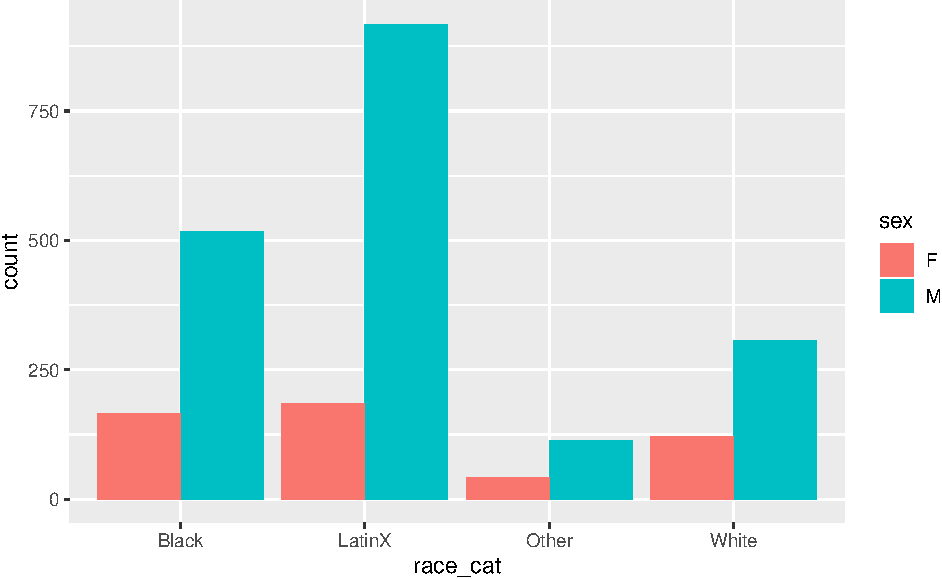
\includegraphics[width=\textwidth]{afam-188r_files/figure-latex/unnamed-chunk-9-1} \end{center}

\hypertarget{variable-distribution}{%
\subsection{Variable distribution}\label{variable-distribution}}

\begin{Shaded}
\begin{Highlighting}[]
\KeywordTok{ggplot}\NormalTok{(arrests, }\KeywordTok{aes}\NormalTok{(}\DataTypeTok{x=}\NormalTok{arrest_time)) }\OperatorTok{+}\StringTok{ }\KeywordTok{geom_histogram}\NormalTok{()}
\end{Highlighting}
\end{Shaded}

\begin{verbatim}
## `stat_bin()` using `bins = 30`. Pick better value with `binwidth`.
\end{verbatim}

\begin{center}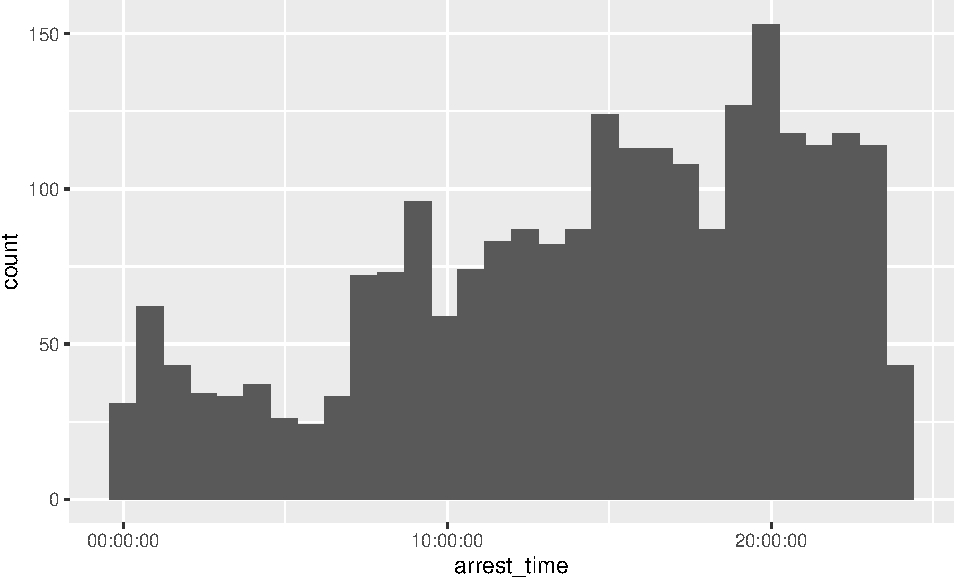
\includegraphics[width=\textwidth]{afam-188r_files/figure-latex/unnamed-chunk-10-1} \end{center}

\hypertarget{two-variables}{%
\subsection{Two variables}\label{two-variables}}

\begin{Shaded}
\begin{Highlighting}[]
\KeywordTok{ggplot}\NormalTok{(arrests, }\KeywordTok{aes}\NormalTok{(}\DataTypeTok{x=}\NormalTok{arrest_type, }\DataTypeTok{y=}\NormalTok{age)) }\OperatorTok{+}\StringTok{ }\KeywordTok{geom_boxplot}\NormalTok{()}
\end{Highlighting}
\end{Shaded}

\begin{center}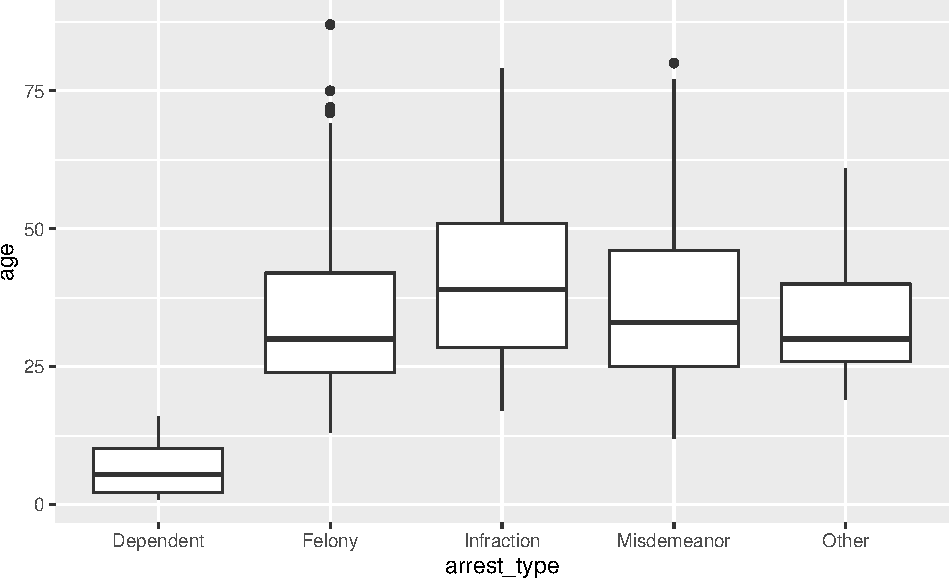
\includegraphics[width=\textwidth]{afam-188r_files/figure-latex/unnamed-chunk-11-1} \end{center}

\hypertarget{ggplot-map}{%
\subsection{Ggplot map}\label{ggplot-map}}

How about we make a map with GGPLOT?

\begin{Shaded}
\begin{Highlighting}[]
\KeywordTok{ggplot}\NormalTok{(arrests, }\KeywordTok{aes}\NormalTok{(}\DataTypeTok{x=}\NormalTok{longitude, }\DataTypeTok{y=}\NormalTok{latitude)) }\OperatorTok{+}\StringTok{ }\KeywordTok{geom_point}\NormalTok{()}
\end{Highlighting}
\end{Shaded}

\begin{center}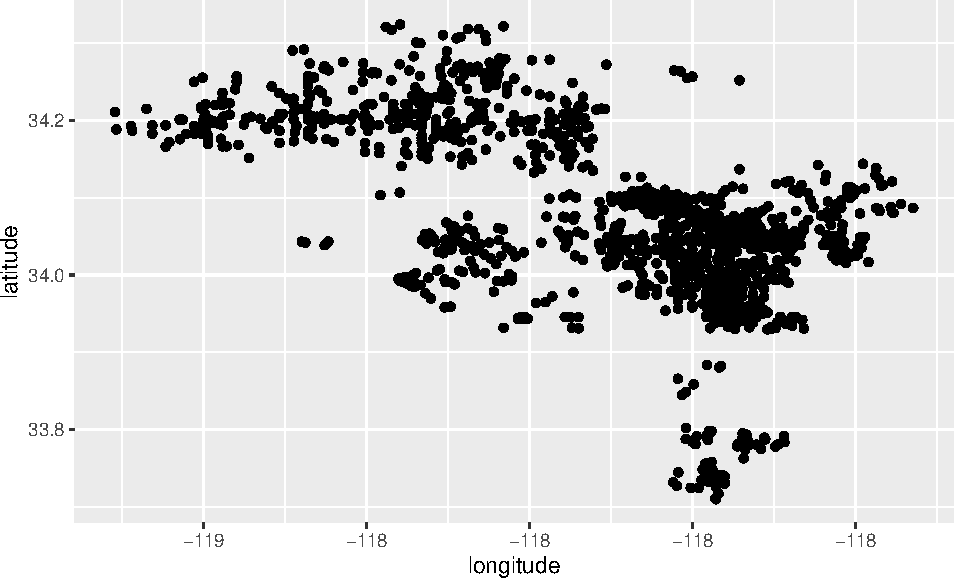
\includegraphics[width=\textwidth]{afam-188r_files/figure-latex/unnamed-chunk-12-1} \end{center}

We can see the general shape of LA, but there are limits to what you can do with geospatial data in ggplot. It doesn't know what to do with the latitude and longitude beyond adding the points to a plot. It has no sense of the layers we used in QGIS. But other R packages gives us this capabilities.

\hypertarget{mapping-in-r}{%
\section{Mapping in R}\label{mapping-in-r}}

The one issue is that we need to tell arrests that it is a spatial object in R. To do that we need to use a few spatial packages. Let's load them.

\begin{Shaded}
\begin{Highlighting}[]
\KeywordTok{library}\NormalTok{(sf)}
\KeywordTok{library}\NormalTok{(tmap)}
\end{Highlighting}
\end{Shaded}

\texttt{sf} stands for spatial features. \texttt{tmap} let's us plot maps like \texttt{ggplot}. Ok, first up, let's convert our \texttt{arrests} data to a spatial feature.

\begin{Shaded}
\begin{Highlighting}[]
\NormalTok{arrests_sf <-}\StringTok{ }\KeywordTok{st_as_sf}\NormalTok{(arrests, }\DataTypeTok{coords =} \KeywordTok{c}\NormalTok{(}\StringTok{"longitude"}\NormalTok{, }\StringTok{"latitude"}\NormalTok{), }\DataTypeTok{crs =} \DecValTok{4326}\NormalTok{)}
\end{Highlighting}
\end{Shaded}

Let's look at this new spatial data frame:

\begin{Shaded}
\begin{Highlighting}[]
\KeywordTok{View}\NormalTok{(arrests_sf)}
\end{Highlighting}
\end{Shaded}

We now have a column called \texttt{geometry} at the end of our data frame. This contains our latitude and longitudes.

One thing nice is that we can use the \texttt{plot()} function to plot our spatial data frame.

\begin{Shaded}
\begin{Highlighting}[]
\KeywordTok{plot}\NormalTok{(arrests_sf)}
\end{Highlighting}
\end{Shaded}

\begin{center}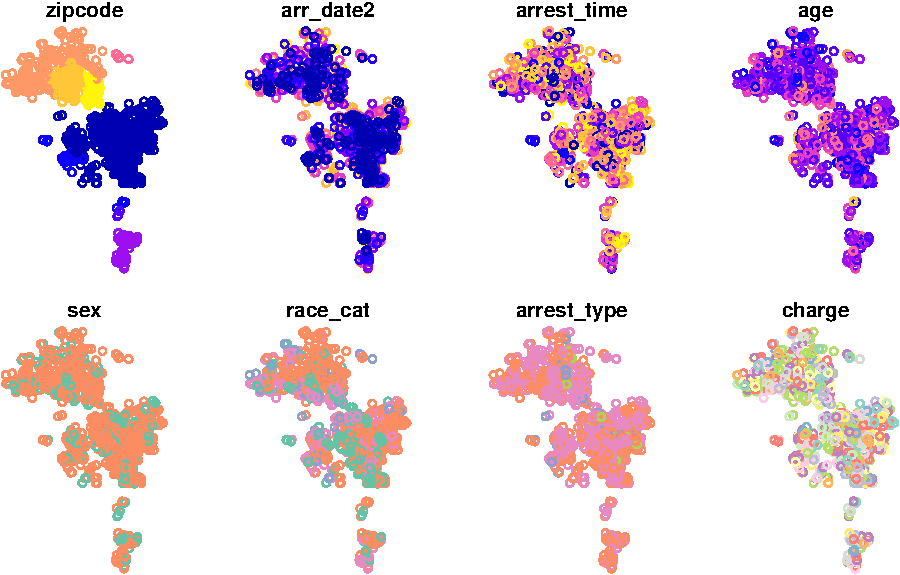
\includegraphics[width=\textwidth]{afam-188r_files/figure-latex/unnamed-chunk-16-1} \end{center}

But the problem is that we still have no context for our points. We need the layers of polygons we had in QGIS to let us know this is LA. Let's look at this in a package called \texttt{tmaps} (thematic maps).

\begin{Shaded}
\begin{Highlighting}[]
\KeywordTok{tm_shape}\NormalTok{(arrests_sf) }\OperatorTok{+}\StringTok{ }\KeywordTok{tm_dots}\NormalTok{()}
\end{Highlighting}
\end{Shaded}

\begin{center}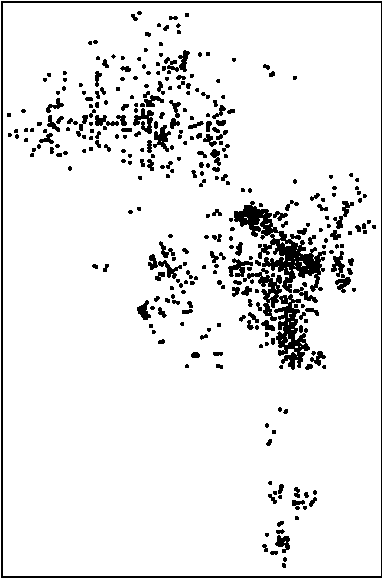
\includegraphics[width=\textwidth]{afam-188r_files/figure-latex/unnamed-chunk-17-1} \end{center}

Nice, but again, we lack geographic boundaries and other shapes. Just like in QGIS, however, we can read in various shapefiles -- the ones ending in \texttt{.shp} -- to provide our map some boundaries. We do this by using the function \texttt{st\_read}. Let's look at our help documentation on \texttt{st\_read}.

Inside our \texttt{data/} folder we have the shape files we used in our \texttt{QGIS} part of the class plus an new one on the LA county boundaries. Let's read them in individually and note the output, especially the \texttt{geometry\ type}.

\begin{Shaded}
\begin{Highlighting}[]
\CommentTok{#geometry type:  MULTILINESTRING}
\NormalTok{la_county <-}\StringTok{ }\KeywordTok{st_read}\NormalTok{(}\DataTypeTok{dsn =}\StringTok{"data/DRP_COUNTY_BOUNDARY/DRP_COUNTY_BOUNDARY.shp"}\NormalTok{)}
\end{Highlighting}
\end{Shaded}

\begin{verbatim}
## Reading layer `DRP_COUNTY_BOUNDARY' from data source `/Users/timdennis/instruction/afam188/afam188-r/data/DRP_COUNTY_BOUNDARY/DRP_COUNTY_BOUNDARY.shp' using driver `ESRI Shapefile'
## Simple feature collection with 2 features and 2 fields
## geometry type:  MULTILINESTRING
## dimension:      XY
## bbox:           xmin: 6280000 ymin: 1380000 xmax: 6670000 ymax: 2120000
## epsg (SRID):    2229
## proj4string:    +proj=lcc +lat_1=35.46666666666667 +lat_2=34.03333333333333 +lat_0=33.5 +lon_0=-118 +x_0=2000000.0001016 +y_0=500000.0001016001 +ellps=GRS80 +towgs84=0,0,0,0,0,0,0 +units=us-ft +no_defs
\end{verbatim}

\begin{Shaded}
\begin{Highlighting}[]
\CommentTok{#geometry type:  MULTIPOLYGON}
\NormalTok{la_zips <-}\StringTok{ }\KeywordTok{st_read}\NormalTok{(}\DataTypeTok{dsn =} \StringTok{"data/Los_Angeles_City_Zip_Codes/Los_Angeles_City_Zip_Codes.shp"}\NormalTok{)}
\end{Highlighting}
\end{Shaded}

\begin{verbatim}
## Reading layer `Los_Angeles_City_Zip_Codes' from data source `/Users/timdennis/instruction/afam188/afam188-r/data/Los_Angeles_City_Zip_Codes/Los_Angeles_City_Zip_Codes.shp' using driver `ESRI Shapefile'
## Simple feature collection with 157 features and 7 fields
## geometry type:  MULTIPOLYGON
## dimension:      XY
## bbox:           xmin: -119 ymin: 33.7 xmax: -118 ymax: 34.3
## epsg (SRID):    4326
## proj4string:    +proj=longlat +datum=WGS84 +no_defs
\end{verbatim}

\begin{Shaded}
\begin{Highlighting}[]
\CommentTok{#geometry type:  MULTILINESTRING}
\NormalTok{la_freeways <-}\StringTok{ }\KeywordTok{st_read}\NormalTok{(}\DataTypeTok{dsn =}\StringTok{"data/CAMS_FREEWAY_SHIELDS/CAMS_FREEWAY_SHIELDS.shp"}\NormalTok{)}
\end{Highlighting}
\end{Shaded}

\begin{verbatim}
## Reading layer `CAMS_FREEWAY_SHIELDS' from data source `/Users/timdennis/instruction/afam188/afam188-r/data/CAMS_FREEWAY_SHIELDS/CAMS_FREEWAY_SHIELDS.shp' using driver `ESRI Shapefile'
## Simple feature collection with 45 features and 4 fields
## geometry type:  MULTILINESTRING
## dimension:      XY
## bbox:           xmin: 6280000 ymin: 1720000 xmax: 6670000 ymax: 2120000
## epsg (SRID):    2229
## proj4string:    +proj=lcc +lat_1=35.46666666666667 +lat_2=34.03333333333333 +lat_0=33.5 +lon_0=-118 +x_0=2000000.0001016 +y_0=500000.0001016001 +ellps=GRS80 +towgs84=0,0,0,0,0,0,0 +units=us-ft +no_defs
\end{verbatim}

Now let's use the layers. The important thing is we match our shapefile with the geometry type. \texttt{tm\_polygons()} goes with \texttt{\#geometry\ type:\ \ MULTIPOLYGON} and \texttt{tm\_line()} goes with \texttt{\#geometry\ type:\ \ MULTILINESTRING}.

\begin{Shaded}
\begin{Highlighting}[]
\KeywordTok{tm_shape}\NormalTok{(la_zips) }\OperatorTok{+}
\StringTok{  }\KeywordTok{tm_polygons}\NormalTok{() }\OperatorTok{+}
\KeywordTok{tm_shape}\NormalTok{(la_freeways) }\OperatorTok{+}
\StringTok{  }\KeywordTok{tm_lines}\NormalTok{() }\OperatorTok{+}
\KeywordTok{tm_shape}\NormalTok{(arrests_sf) }\OperatorTok{+}
\StringTok{  }\KeywordTok{tm_dots}\NormalTok{() }
\end{Highlighting}
\end{Shaded}

\begin{center}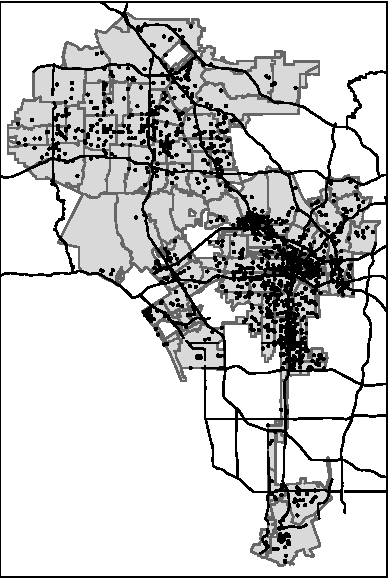
\includegraphics[width=\textwidth]{afam-188r_files/figure-latex/unnamed-chunk-18-1} \end{center}

\begin{Shaded}
\begin{Highlighting}[]
\KeywordTok{tm_shape}\NormalTok{(arrests_sf) }\OperatorTok{+}
\StringTok{  }\KeywordTok{tm_polygons}\NormalTok{(la_county) }\OperatorTok{+}
\StringTok{  }\KeywordTok{tm_dots}\NormalTok{()}
\end{Highlighting}
\end{Shaded}

\hypertarget{mapping-in-r-tmaps-continued}{%
\chapter{Mapping in R: tmaps continued}\label{mapping-in-r-tmaps-continued}}

Class 2, Nov.~18.

\hypertarget{mapping-with-r}{%
\chapter{Mapping with R}\label{mapping-with-r}}

We describe our methods in this chapter.

\hypertarget{mapping-with-r-1}{%
\chapter{Mapping with R}\label{mapping-with-r-1}}

\bibliography{book.bib,packages.bib}


\end{document}
